%!TEX program = xelatex
%!TEX output_directory = out
%!TEX jobname = Thesis Draft Tiebreak (22107 and 22584)
\documentclass[a4paper,11pt]{article}

\usepackage[a4paper,margin=3.5cm,top=3cm,bottom=3cm,footskip=1.5cm]{geometry}

% Import most packages and options
\usepackage{article-style}

% Language and bib options
\DeclareLanguageMapping{american}{american-apa}
\addbibresource{bibliography.bib}
\defbibheading{bibliography}[\refname]{\section*{#1}}

\setmainfont{Minion Pro}

% Title and author and date
\title{Risk analysis of factor strategies: \\A copula approach}
\author{
  \begin{tabular}[t]{@{}c@{}}
    Gustaf Soldan\\
    {\href{mailto:22107@student.hhs.se}{22107@student.hhs.se}}
  \end{tabular}
  \hskip 1em
  \begin{tabular}[t]{@{}c@{}}
    Victor Andrée\\
    {\href{mailto:22584@student.hhs.se}{22584@student.hhs.se}}
  \end{tabular}
}
\date{\textsc{Draft 2: ``Tiebreak''} \\
November XX, 2016}

% Main document pasted from other files
\begin{document}
\maketitle
\begin{abstract}
We evaluate diversification in factor strategies using a dynamic copula approach.
\end{abstract}
\pagebreak
%!TEX root = ../main.tex
\section{Introduction}
\textcite{FF2015} find that the value factor, HML, is redundant in a four-factor model including profitability (RMW) and investment (CMA), as it has no explanatory power on monthly returns in a US 1963–2010 sample. This could mean that the classic value factor is an inferior proxy for what truly comprises value. This paper takes a risk perspective on factor equity strategies and investigates what role HML has in factor investing, given the discovery of RMW and CMA. 

How can it be that HML is subsumed by CMA and RMW? [While most factor pairs exhibit relatively low correlation, the CMA and HML pair stands out with an unconditional correlation in our sample period of approx. 0.60, indicating a much higher similarity between these two factors. For a factor pair that has this high correlation coefficient, we believe that it is important to analyze whether they are both neccessary in a portfolio, regardless of whether they add alpha or not. Furthermore, HML is value minus growth and CMA is asset reduction minus asset growth. Naturally, there could be a connection between the growth valuation component in HML and the asset growth component of CMA, and it is not surprising that there is some overlap in the component stocks [what does previous research. We therefore give extra weight to analysis on how CMA and HML relates to eachother and to a factor portfolio as a whole.]

While analyses could be made on sample data alone, we wish to thoroughly examine factors by building a conditional model of return series, that can incorporate dependencies that are otherwise hard to capture in sample data, such as time-varying correlations and tail dependence. Tail dependence is the notion that there might be significantly different dependence patterns when returns simultaneously realize in the lower or upper tail, as opposed to close to the center of the distribution. From previous research on factors~\autocite{ChristoffersenLanglois2013}, we have reason to believe that the factor strategies exhibit both tail dependence and dynamic correlations, and show that this is the case also for RMW and CMA.

Recently, copula models have attracted considerable attention in the risk management field, as they offer a numerically feasible and flexible way of estimating joint probability distributions. From a copula model, we are able to simulate one-week ahead conditional forecasts of the return series. More specifically, a copula model can be estimated with univariate models as a starting point. First, we examine the factor return series on a univariate level and find evidence of autocorrelation and volatility clustering, in line with stylized facts on financial return series, and specify univariate models from the ARMA-GARCH family to capture these dynamics. The ARMA-GARCH models achieve white noise residuals for each factor, but we show that there is still substantial dependence between the residual series, indicating multivariate dependence. The copula then uses the residual series from these models and tries to explain the interdependence. The main advantage of using a copula is that it is flexible enough to generate tail dependence as well as dynamic correlations, and might improve on the description of return series.

We revisit the regressions of \textcite{FF2015} that show a zero alpha of including HML in a four-factor portfolio of Mkt-RF, SMB, RMW and CMA, but replace monthly data with weekly data and include the momentum factor. Weekly data gives a more granular understanding of risk, as shocks are more smoothed on a monthly basis. Momentum is also included, as it is frequently used in factor equity investing.\footnote{See i.a. \textcite{Pedersen2015}, \textcite{Ilmanen2011}} 

We then test the conjecture in \textcite{FF2015} that the insignificant alpha of adding HML to a four-factor portfolio implies that a mean-variance investor should in fact not include HML in her portfolio. By saving a third of the data for out-of-sample analysis, we re-estimate the copula model and construct mean-variance optimal portfolios and study the optimal weights over time. In the mean-variance analysis, we can also quantify the Sharpe ratios of portfolios including and excluding HML and CMA respectively. In addition to Sharpe ratios, we quantify higher moment risk measures of competing portfolios, including skewness and maximum drawdown. Furthermore, the out-of-sample investing investigates the performance of different copula specifications. Do conditional and asymmetric models improve the Sharpe ratio? And what happens to other risk measures?

Finally, we study the diversification benefits of HML, RMW and CMA respectively, based on simulations from a model of joint returns. More specifically, we take the copula model of factor returns as given and investigate how close the expected shortfall of a factor portfolio can come to the theoretical optimum, which is the same portfolio's Value-at-Risk. This statistic, the conditional diversification benefit (CDB) is due to \textcite{ChristoffersenErrunzaJacobLanglois2012}, and can, in the model setting, shed light on the relative benefits of including one of the similar factors HML or CMA, respectively.

___

Tease a little results
 
___

The structure of this thesis is as follows: in \autoref{sec:2} we provide a brief literature review of factor strategies and the work on copulas relating to factors. In \autoref{sec:3} we present the data used and detail the construction of factors. In \autoref{sec:4} we present the main empirical analysis by interleaving method and results. In \autoref{sec:5} we summarize our findings and discuss their wider implications.
\pagebreak
%!TEX root = ../main.tex
\section{Literature review}
\label{sec:literature}
\textcite{FF2015} introduce two additional factors to complement the \textcite{FamaFrench1993} three-factor asset pricing model. In what is referred to as the five-factor model, the traditional factors (market, value and size) are complemented by a profitability factor and an investment factor. Both factors represent zero-cost portfolios: the profitability factor, denoted RMW (robust-minus-weak), is long firms with high operating profitability and short firms with low operating profitability, and the investment factor, denoted CMA (conservative-minus-aggressive), is long firms with low investment rate and short firms with high investment rate. The five-factor model is found to be a siginificant improvement over the three-factor model, and the two new factors appear to have made the value factor, HML (high-minus-low), redundant. More specifically, the authors show that there is no significant intercept in regressions of HML on the remaining four factors, while each of the other factors have significant intercepts in similar regressions. The high average return of the HML factor appears to be fully explained by the remaining four factors. In an investment context, this can be interpreted as the HML factor adding no alpha to a portfolio holding the remaining four factors.

\textcite{Asness2015} challenge the notion that the value factor is subsumed by the addition of investment and profitability. In their study, they add a momentum factor, as well as an enhanced HML factor, and resurrect the alpha of the value factor. This leads us to believe that momentum could play an important role in recognizing the effect of HML. The momentum factor was originally studied by \textcite{JegadeeshTitman1993} and has since been shown to be present in many financial return series~\autocite{AsnessMoskovitzPedersen2013}.

It is debated whether factor strategies constitute rational risk premia or whether they are the consequences of market imperfections and irrational behavior. There are some appealing rational stories for the return premium of HML. \textcite{FamaFrench1993} show that the HML factor is related to systematic patterns of profitability and growth, and could proxy for a common risk source. This is supported by \textcite{LiewVassalou2000}, who show that the value factor can predict real GDP growth on data in several markets. \textcite{Zhang2005} uses a neoclassical model with rational expectations and competitive equilibrium to show that value firms have more tangible assets and are burdened by industry over-capacity in downturns, leading to higher down-market betas. \textcite{PetkovaZhang2005} find that the conditional betas of value stocks covary positively with the expected market risk premium.

Despite there being a number of rational theories, they all predict effects that are fairly small and cannot fully motivate the value premium. So far, the most pervasive explanations of the value premium are based on market imperfections and irrational behavior.\footnote{See i.a. \textcite{Ilmanen2011}}

\textcite{LakonishokShleiferVishny1994} argue that the value factor is driven by investors' overreaction to changes in earnings. They show that value firms have often experieced a decline in earnings over the last three years, lowering their book to market ratio. When earnings have gone down, investors as a group extrapolate the trend into the future and push prices away from fundamentals, giving rise to higher average returns for value firms and vice versa. Similar to \textcite{LakonishokShleiferVishny1994}, \textcite{BarberisHuang2001} draw on the fact that value firms have experienced decreasing earnings, but suggest that the premium is driven by investors' loss aversion bias. Current value firms have had falling earnings, leading to lower share prices and negative returns. As investors are deterred by the past performance of negative returns in itself, they are less willing to hold value stocks. \textcite{LakonishokShleiferVishny1992} instead find an explanation in the structure of the money manager industry. They suggest that there money managers have career based incentives to avoid value stocks as such stocks are more likely to go bankrupt, and make the short-term performance look bad, than growth stocks, which are more widely held in the reference index.

Variations of the long-short strategy of the value factor has become a staple strategy of both quantitative and qualitative hedge funds, often under the "equity market neutral" or "fundamental quantitative" labels. Factor equity strategies have also become increasingly accessible for retail investors, especially with the advent of smart beta ETFs. \footnote{See i.a. \textcite{Pedersen2015}, \textcite{AQREMN} and \textcite{McKEMN}.} 

The use of leverage in hedge funds can exacerbate the flow patterns in factor strategies, as highlighted by the quant crash in July-August 2007. \textcite{KhandaniLo2011} and \textcite{KhandaniLo2007} revisit the sudden and large losses of factor strategies (including value and size) during this period, and provide evidence for the "Unwind hypothesis": The crash started with rapid sell-offs of large blocks of factor strategy portfolios, for which there was not enough liquidity to maintain prices. The price drops, in turn, led to further liquidations due to 1) margin calls in other leveraged and long-short funds and 2) risk management policies, even in traditional long-only funds. This liquidity and margin spiral is very similar to that proposed by \textcite{Brunnermeier2009} and \textcite{BrunnermeierPedersen2009}.

Other papers have also highlighted the risk of "crowded trades" where leverage is applied. \textcite{Stein2009} shows that markets can become less pricing efficient and have increased chances of large fire-sale crashes when rational investors set their leverage level unknowing of how many others are engaging in a similar trade. \textcite{LouPolk2013} introduce measures of arbitrage activity and show that momentum strategies become destabilizing and prone to crash in times of high activity. For the value strategy, high arbitrage activity is instead shown to forecast positive value returns. 

The profitability and investment factors have only recently made their way into academic literature. \textcite{NovyMarx2013} study the return differences between firms with high and low gross profitability and shows significant abnormal returns to a profitability factor. Profitability is also shown to have approximately the same power in predicting the cross-section of stock returns as does value (book-to-market). Furthermore, the profitability strategy is negatively correlated with value, and can therefore improve the investing performance of a value strategy. \textcite{CooperGulenSchill2008} investigate investment, measured as the percentage change in total assets, and show that the related zero-cost-portfolio provides significant abnormal returns and that it has additional predictive ability in the cross-section of stock returns, taking both value and size into account.

While all other factor pairs are nearly uncorrelated or negatively correlated, the value (HML) and investment (CMA) factors are highly positively correlated. \textcite{Zhang2005} predicts this positive relation in a model setting, and \textcite{AndersonGarciaFeijoo2006} confirm it on empirical data. More specifically, the empirical study shows that past investment has a significant positive relation with the book-to-market ratio. In other words, value firms with high book-to-market might be value firms precisely because they have invested little, and vice versa. \textcite{FF2015} consider it a fact that value firms invest less than growth firms.

There are only a handful of papers that study factor strategies using copula methods. A working paper by \textcite{CholleteNing2012} examine dynamic correlations between a four-factor model and aggregate US consumption, and find evidence for tail dependence across the five risk factors. \textcite{ChristoffersenLanglois2013} study the four-factor model alone on US data 1963-2010, and show significant and asymmetric tail dependence that cannot be captured by standard linear correlation measures. A skewed Student-\textit{t} copula-GARCH model is found to be able to generate the model fairly well, and the authors proceed with 20 years of out-of-sample analysis on investing based on conditional expectations from the copula model, leading to significant improvements for investors with a CRRA utility function. To the best of our knowledge, no paper has previously studied the role of the investment and profitability factors using copula models.
\pagebreak
%!TEX root = ../main.tex
\section{Data}
\label{sec:data}
In the data section, we describe the source of our data and how the factor strategies are constructed. We then present summary statistics including tests for serial correlation and volatility clustering, as well as quantile-quantile (QQ) plots. Finally, we discuss the unconditional correlation of the factor strategies.

\subsection{Data description: Factor return series}

Factor return series are downloaded from Ken French's data library.\footnote{Ken French Data Library. (2016). \textit{Fama/French 5 Factors (2x3) [Daily]} and \textit{Momentum Factor (Mom) [Daily]}. Available from: \url{http://mba.tuck.dartmouth.edu/pages/faculty/ken.french/data_library.html}} We download the daily Fama-French five-factor data set and merge this with the daily momentum data set. Both are available since 1963-07-01, making 1963-07-05 the first week of data. In our sample, 2016-07-01 is the last data point. We convert each of the return series into weekly log returns for further use. 

The Mkt-RF factor is long the value-weighted return of CRSP firms on NYSE, AMEX or NASDAQ with CRSP share codes 10 or 11 and short the one-month Treasury bill rate. The remaining return series are based on zero-cost portfolios that are long certain equities and short other equities, according to a 2 x 3 sort: First, firms are sorted into one of two size groups, small and big, depending on whether the market cap is above or below the median. In the small and big firm groups, each factor then sorts into one of three groups depending on whether the variable of interest falls below the 30\textsuperscript{th} percentile, between the 30\textsuperscript{th} and the 70\textsuperscript{th} or above the 70\textsuperscript{th}. For the five-factor data set, the factors are:
\begin{itemize}
  \item High-minus-low, is long firms above the 70\textsuperscript{th} percentile B/M (high) and short stocks below the 30\textsuperscript{th} percentile, in the small and big firm group respectively. \\
  $HML = 1/2 \cdot (Small\,value + Big\,value) - 1/2 \cdot (Small\,growth + Big\,growth)$
  \item Small-minus-big, is long firms below the 50\textsuperscript{th} percentile market cap and short firms above the 50\textsuperscript{th} percentile, in each of three groups. \\
  $SMB = 1/3 \cdot (SMB_{HML} + SMB_{RMW} + SMB_{CMA}$)
  \item Robust-minus-weak, is long firms above the 70\textsuperscript{th} percentile operating profitability and short firms below the 30\textsuperscript{th} percentile. \\
  $RMW = 1/2 \cdot (Small\,robust + Big\,robust) - 1/2 \cdot (Small\,weak + Big\,weak)$
  \item Conservative-minus-aggressive, is long firms above the 70\textsuperscript{th} percentile total asset growth and short firms below the 30\textsuperscript{th} percentile. \\
  $CMA = 1/2 \cdot (Small\,conservative + Big\,conservative) - 1/2 \cdot (Small\,aggressive + Big\,aggressive)$
\end{itemize}
The sort ensures that SMB includes firms small and big firms equally from the other factors, and that the other factors include equal amounts of small and big firms. Note that momentum originates from a different data set and does not affect the SMB compisition.
\begin{itemize}
  \item Momentum, is long firms above the 70\textsuperscript{th} percentile prior 2-12 month return (i.e. excluding the last month) and short stocks below the 30\textsuperscript{th} percentile, in the small and big firm group respectively. \\
  $Mom = 1/2 \cdot (Small\,high + Big\,high) - 1/2 \cdot (Small\,high + Big\,high)$
\end{itemize}
French's financial statement data originates from Compustat, stock return data from CRSP and Treasury return data from Ibbotson Associates.

\subsection{Summary statistics}
% Table created by stargazer v.5.2 by Marek Hlavac, Harvard University. E-mail: hlavac at fas.harvard.edu
% Date and time: lör, okt 15, 2016 - 22:22:53
\begin{table}[!htbp] \centering 
  \caption{Summary statistics of data} 
  \label{tab:summarydata} 
\begin{tabularx}{\textwidth}{X}
  \\[-1.8ex]%\toprule
  \\[-1.8ex] 
  \footnotesize Summary statistics of weekly log returns on factor strategies. Kurtosis is excess kurtosis, standardized to zero. LB [5/10] is the weighted Ljung-Box test up to 5/10 lags of \textcite{FisherGallagher2012}, where the null hypothesis is no autocorrelation.
\end{tabularx}
\begin{tabularx}{\textwidth}{@{\extracolsep{5pt}} X r r r r r r} 
  \\[-1.8ex]\midrule
  \\[-1.8ex] 
  & Mkt.RF & SMB & Mom & HML & CMA & RMW \\ 
\hline \\[-1.8ex] 
Observations & $2,766$ & $2,766$ & $2,766$ & $2,766$ & $2,766$ & $2,766$ \\ 
Maximum & $0.126$ & $0.060$ & $0.120$ & $0.117$ & $0.054$ & $0.094$ \\ 
Minimum & $$-$0.198$ & $$-$0.098$ & $$-$0.175$ & $$-$0.083$ & $$-$0.044$ & $$-$0.062$ \\ 
Mean & $0.001$ & $0.000$ & $0.001$ & $0.001$ & $0.001$ & $0.001$ \\ 
Median & $0.003$ & $0.001$ & $0.002$ & $0.000$ & $0.000$ & $0.000$ \\ 
Volatility & $0.022$ & $0.012$ & $0.019$ & $0.012$ & $0.009$ & $0.009$ \\
Skewness & $$-$0.688$ & $$-$0.504$ & $$-$1.390$ & $0.331$ & $0.306$ & $0.724$ \\ 
Kurtosis & $6.191$ & $4.997$ & $11.987$ & $7.318$ & $3.149$ & $13.005$ \\
\\[-1.8ex]\hline
  \\[-1.8ex] 
Return LB [5] p-value & $0.263$ & $0.000$ & $0.000$ & $0.000$ & $0.000$ & $0.000$ \\ 
Return LB [10] p-value & $0.007$ & $0.000$ & $0.000$ & $0.000$ & $0.000$ & $0.000$ \\ 
Return\textsuperscript{2} LB [5] p-value & $0.000$ & $0.000$ & $0.000$ & $0.000$ & $0.000$ & $0.000$ \\ 
Return\textsuperscript{2} LB [10] p-value & $0.000$ & $0.000$ & $0.000$ & $0.000$ & $0.000$ & $0.000$ \\ 
%\bottomrule \\[-1.8ex] 
\end{tabularx} 
\end{table}
For all series, there are 2,766 consecutive data points and no missing data. Mkt-RF is the most volatile and extreme of the series, with weekly returns between -19.8\% and 12.6\% and a standard deviation of 2.2\%. Among the value strategies, CMA and RMW seem to be less extreme than HML, with less negative minimums and smaller standard deviations. The factor strategies have excess kurtosis, or fat tails, that is typical for financial returns. The excess kurtoses of the Mom, HML and RMW factors are even higher than the kurtosis of the Mkt-RF factor. However, while market returns are negatively skewed, the value strategies HML, CMA and RMW instead exhibit positive skewness. QQ-plots versus normal theoretical quantiles in \autoref{fig:qq_returns} graphically show the non-normality.
\begin{figure}[H]
  \caption{QQ-plots versus normal distribution}
  \label{fig:qq_returns}
  %\toprule
  \centering
  \begin{minipage}{\textwidth}
  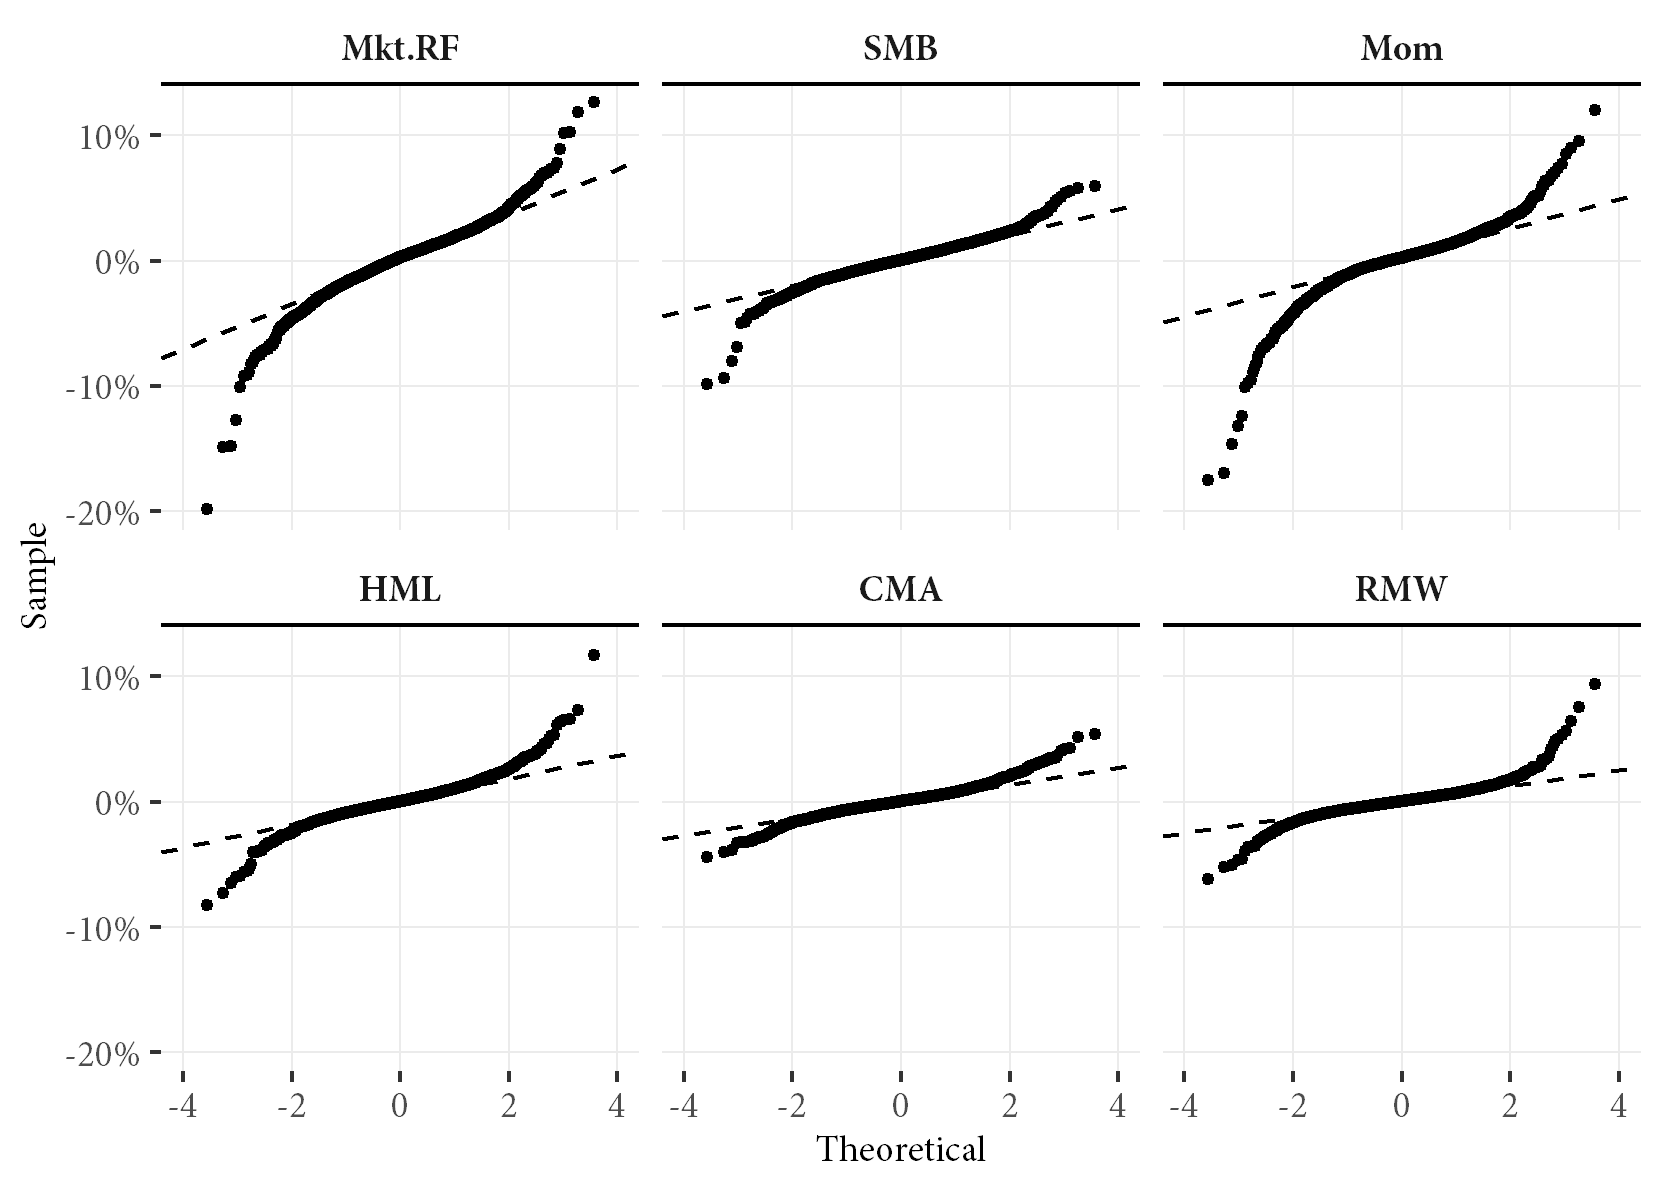
\includegraphics[scale=1]{graphics/qq_returns.png}  
  %\bottomrule
  \vspace{3mm}
  \footnotesize
  Quantile-quantile plots of theoretical (normal) and sample quantiles. Data from a normal distribution should line up on the dashed line. Weekly log returns 1963-2016
  \end{minipage}
\end{figure}


We conduct Ljung-Box tests of the factor returns to control for weekly autocorrelation.\footnote{For a detailed description of the test, see \autoref{sub:diagnostic_test_procedures}} The p-values of these tests are given in \autoref{tab:summarydata} and are very low for all factors except Mkt-RF, leading to a strong rejection of the zero autocorrelation null hypothesis. For Mkt-RF, the p-value is not enough for a rejection of zero autocorrelation at the 5 week maximum lag length, but strongly rejected for 10 weeks of maximum lags. We also conduct Ljung-Box tests of the squared factor returns to control for volatility clustering (ARCH effects). Here, the null hypothesis is that there are no ARCH effects, and p-values given in \autoref{tab:summarydata} strongly rejects the null for all factors at both max lag length of 5 and 10.

We conclude that factor return series are non-normal and exhibit both autocorrelation as well as autoregressive heteroscedasticity. These predictable phenomena in financial return data are typically captured by models that incorporate autoregressive components for both the conditional mean and variance equations, such as the family of ARMA-GARCH models, which are further discussed in \autoref{sec:univariate_modeling}.
\begin{figure}[H]
  \caption{Cumulative returns to factor strategies}
  \label{fig:cumret}
  %\toprule
  \centering
  \begin{minipage}{\textwidth}
  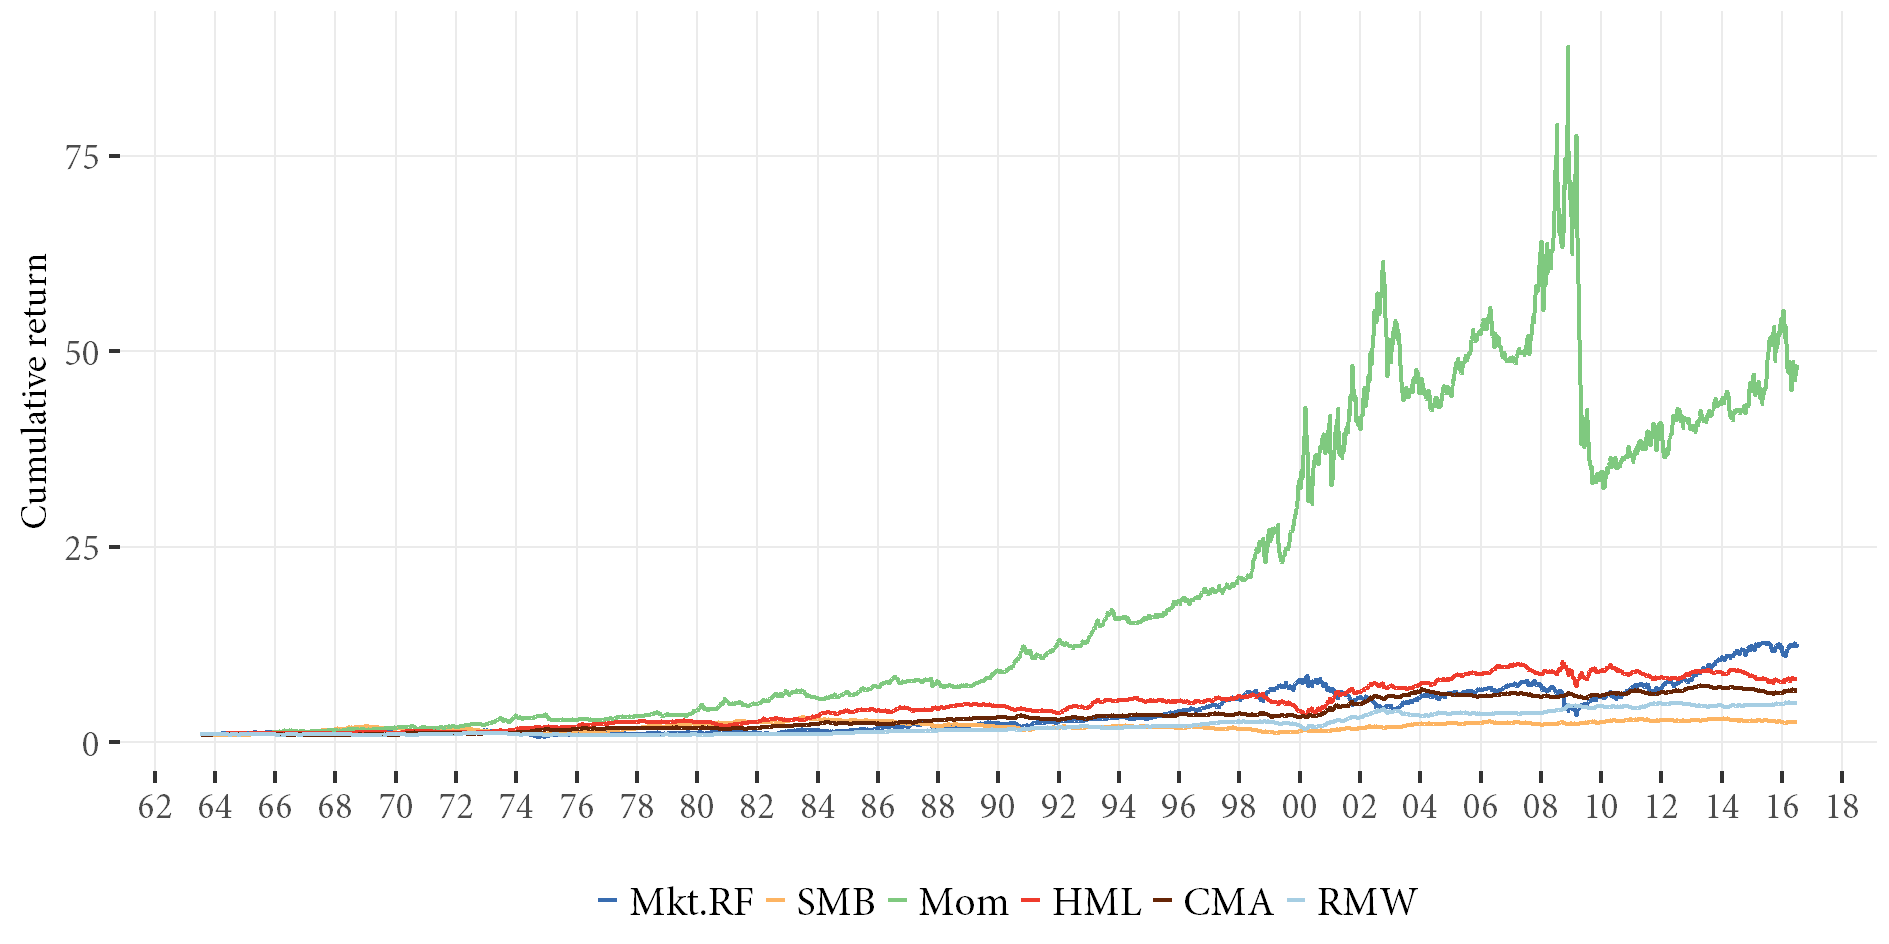
\includegraphics[scale=1]{graphics/cumretPlot.png}  
  %\bottomrule
  \vspace{3mm}
  \footnotesize
  Cumulative returns to investing one dollar in each factor strategy beginning 1963-07-05.  All data 1963-07-05 - 2016-07-01.
  \end{minipage}
\end{figure}
\begin{figure}[H]
  \caption{Standardized cumulative returns to factor strategies}
  \label{fig:cumretstd}
  %\toprule
  \centering
  \begin{minipage}{\textwidth}
  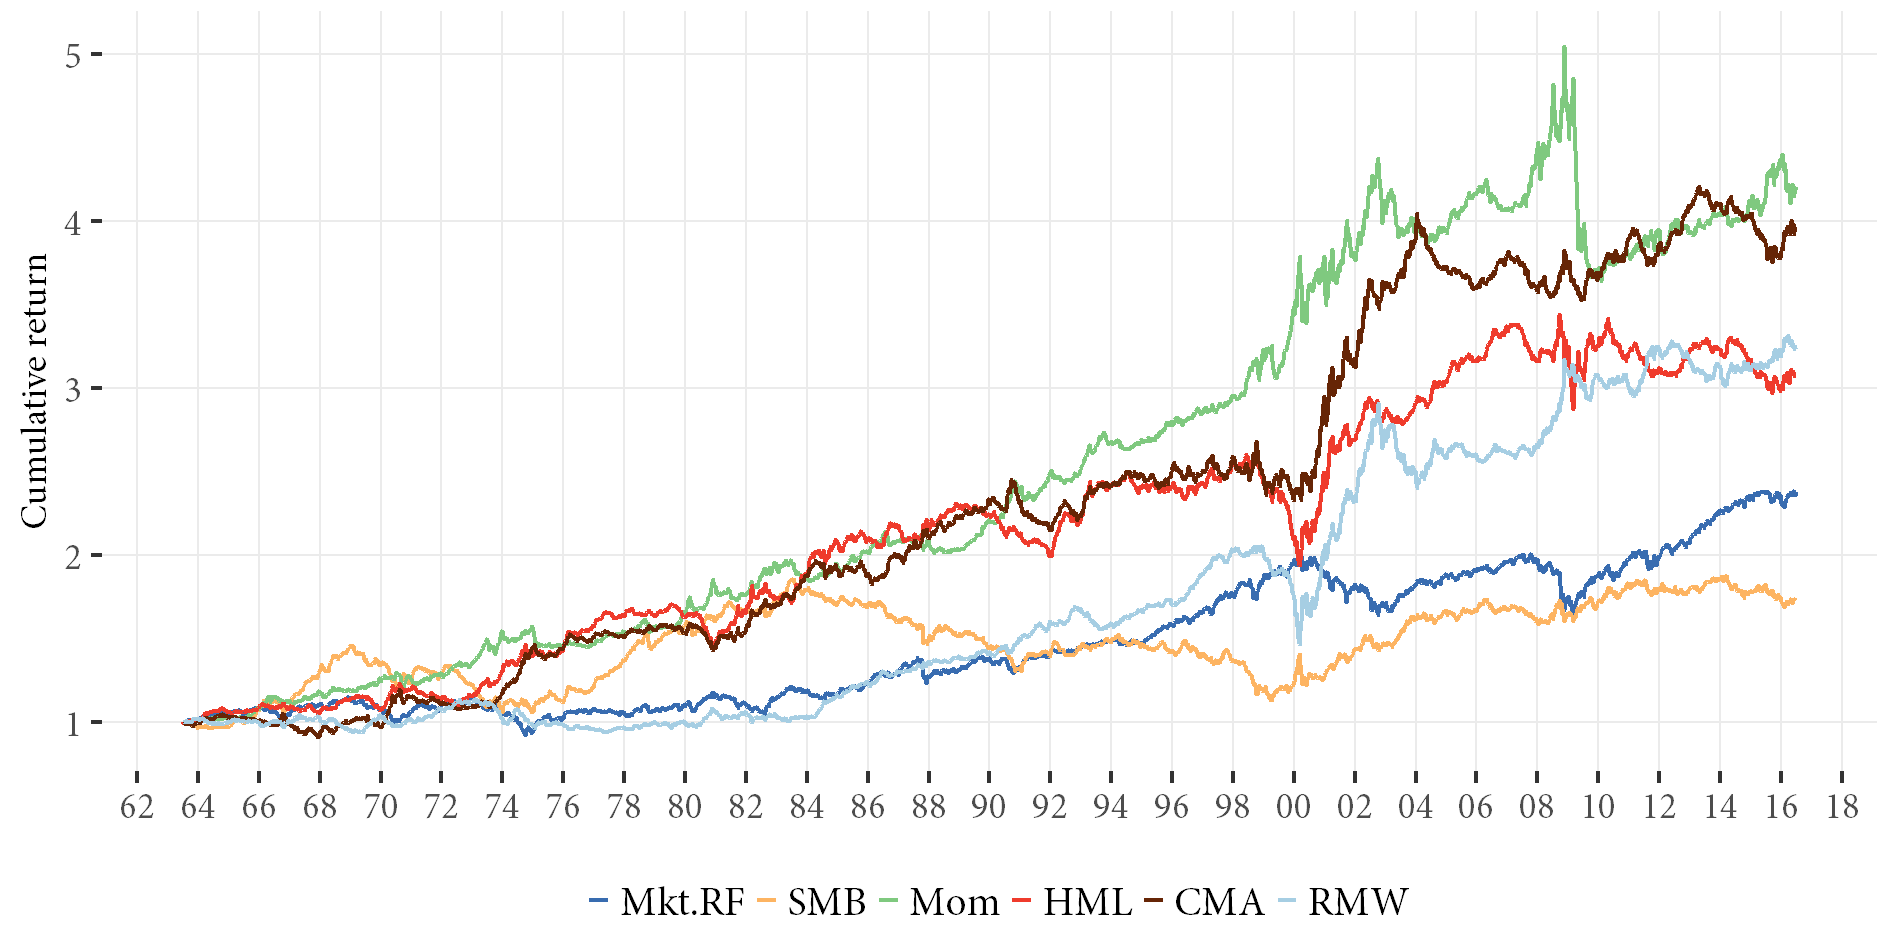
\includegraphics[scale=1]{graphics/cumretStdPlot.png}  
  %\bottomrule
  \vspace{3mm}
  \footnotesize
  Cumulative returns to investing one dollar in each factor strategy beginning 1963-07-05. Standardized to 10\% annual volatility. All data 1963-07-05 - 2016-07-01.
  \end{minipage}
\end{figure}

Plots of cumulative returns (\autoref{fig:cumret}) clearly show the high returns to the momentum strategy through the sample period. However, normalizing the series to 10\% annual volatility (\autoref{fig:cumretstd}) gives a more nuanced picture of mean-variance performance. Since 1963, each of the strategies except for SMB has outperformed the market factor. Furthermore, factor strategies seem to crash at different times and diversify eachother, e.g. Mom performing well during 1999-2000 and RMW performing well during 2008-2009. The unconditional correlation matrix of returns is given in \autoref{tab:corr_matrix} and the general low or even negative correlation coefficients show the diversification benefits of factor strategies. The HML - CMA pair does stand out, however, with an unconditional correlation of 0.625, which could be related to a partial overlap of the factor components as discussed in \autoref{sec:literature} -- past investment is shown to be positively empirically related to the current book-to-market ratio. The substantially higher correlation in this asset pair indicates lower diversification benefits between the two strategies and begs the question whether both should be included in a factor portfolio.

\begin{table}[!htbp] \centering 
  \caption{Correlation matrix} 
  \label{tab:corr_matrix} 
\begin{tabularx}{\textwidth}{X}
  \\[-1.8ex]%\toprule
  \\[-1.8ex] 
  \footnotesize Unconditional sample correlation matrix of factor log return series. Weekly data 1963-2016
\end{tabularx}
\begin{tabularx}{\textwidth}{@{\extracolsep{5pt}} X r r r r r r} 
  \\[-1.8ex]\midrule
  \\[-1.8ex] 
  & Mkt.RF & SMB & Mom & HML & CMA & RMW \\ 
\hline \\[-1.8ex] 
Mkt.RF & $1.000$ & $$ & $$ & $$ & $$ & $$ \\ 
SMB & $0.086$ & $1.000$ & $$ & $$ & $$ & $$ \\ 
Mom & $$-$0.113$ & $$-$0.007$ & $1.000$ & $$ & $$ & $$ \\ 
HML & $$-$0.283$ & $$-$0.026$ & $$-$0.219$ & $1.000$ & $$ & $$ \\ 
CMA & $$-$0.416$ & $$-$0.048$ & $0.071$ & $0.625$ & $1.000$ & $$ \\ 
RMW & $$-$0.154$ & $$-$0.337$ & $0.080$ & $$-$0.054$ & $$-$0.067$ & $1.000$ \\ 
%\bottomrule \\[-1.8ex] 
\end{tabularx} 
\end{table}
\pagebreak
%!TEX root = ../main.tex

\section{Modeling Factor Returns} % (fold)
\label{sec:modeling_factor_returns}

We proceed by estimating models of each factor's return series, trying to capture the established effects of serial correlation, volatility clustering, non-normality and leverage effects in financial returns. By estimating appropriate models, we can characterize and filter these effects, while incorporating them in conditional forecasts. In this section, we describe the general structure of our models, our systematic model selection approach and estimation results.

\subsection{General univariate model: ARMA-GJR-GARCH} % (fold)
\label{sub:general_univariate_model_gjr_garch}

The ARMA-GARCH is a broad model family designed to eliminate predictable components of financial return series. The models use autoregressive and moving average lags to capture serial correlation in return data (ARMA), as well as autoregressive and moving average lags to capture ARCH effects in residuals from the mean equation (GARCH). ARCH effects are also referred to as volatility clustering, due to the persistence in magnitude of return shocks. Shocks in financial return series are often not homoskedastic, and the hetreoskedasticy tends to exhibit serial correlation. We evaluate the GJR-GARCH model of~\textcite{glosten1993relation}, which is a parsimonious extension of the standard GARCH(1, 1) model of~\autocite{Bollerslev1986}. The GJR-GARCH is designed to also capture leverage effects~\autocite{glosten1993relation}, i.e. when negative and positive return shocks have different impact on future volatility~\autocite{Black1976}.

We estimate conditional mean equations \emph{up to} ARMA(3, 3):
\begin{align}
  r_t &=
    \mu +
    \sum^p \phi_p r_{t - p} +
    \sum^q \theta_q \epsilon_{t - q} + 
    \epsilon_t
\end{align}
where $r_t$ are log returns. The conditional volatility evolves according to the GJR-GARCH specification:
\begin{align}
  \epsilon_t &= \sigma_t z_t \\
  \sigma_t^2 &=
    \omega +
    (\alpha + \eta I_{\epsilon_{t-1} \leq 0}) \epsilon_{t - 1}^2 +
    \beta \sigma^2_{t - 1}
\end{align}
where $I$ is an indicator function that is equal to one when $\epsilon_{t-1} \leq 0$. A positive $\eta$ captures the leverage effect by increasing the current period's volatility if the previous period's residual $\epsilon$ was below zero. A significant $\eta$ thus introduces asymmetric volatility in the model. For the market factor, it is expected that $\eta$ is positive, reflecting the leverage effect in the market itself and no impact from the short risk-free component. However, for the other factors, which are constructed as all-equity zero-cost long-short portfolios, the direction of $\eta$ is less obvious~\autocite{ChristoffersenLanglois2013}. If there are leverage effects for stocks in general, negative shocks will lead to more volatility than positive shocks in a portfolio of stocks. But in a zero-cost portfolio, the leverage effects of the long positions in stocks could be eliminated by the short positions in other firms. The level of the leverage effect in a zero-cost portfolio therefore depends on the relative strength of leverage effects in the long and short components.

The ARMA-GARCH models are estimated on each series using maximum likelihood estimation, taking an assumed conditional distribution of standardized returns $\{z_t\}$ as given. We evaluate models where the standardized residuals series $\{z_t\}$ are assumed to follow one of the following distributions: Standard normal, Student's \textit{t} with $\nu$ degrees of freedom and skewed Student's \textit{t} with $\nu$ degrees of freedom and skewness $\gamma$. The Student's t distribution allows for greater kurtosis (fatter tails) than the standard normal distribution, while skewed Student's \textit{t} also allows for additional asymmetry in the model's behavior beyond that introduced by the leverage effect. In the estimation, we also use variance targeting as proposed by~\textcite{EngleMezrich1995}, which is shown makes optimization faster and sometimes more certain to reach the global maximum. This means that $\omega$ is not estimated in the maximum likelihood setting, but instead set to 1 minus the persistence of the process times the sample mean of squared residuals, where the persistence is $\alpha + \beta$ for the GARCH.\footnote{Note that in the case of the GJR-GARCH for the Mkt-RF factor, the persistence is $\alpha + \beta + \eta \kappa$ where $\kappa$ is the probability that standardized residuals $z_t$ are below zero.}

% subsection general_univariate_model_gjr_garch (end)

\subsection{Selection Process} % (fold)
\label{sub:selection_process}

Our estimation process is as follows: For each factor strategy, we estimate GJR-GARCH models on the full dataset ($T = 2766$) up to ARMA(3, 3) and GARCH(1, 1) under normal, Student's t and skewed Student's t residuals, with and without $\eta$ fixed to zero (in which case we obtain the basic GARCH(1, 1) model). We then compute the Bayesian Information Criterion (BIC~\autocite{Schwarz1978}) for each factor strategy and specification and select the ARMA order with the lowest BIC as our primary candidates.

First, the candidate models are checked for remaining serial correlation and ARCH effects. Second, we examine whether there are significant leverage effects that warrant the use of a GJR-GARCH instead of a standard GARCH. Third, we use QQ-plots to control for misspecification in the residual process, and to find a suitable distribution for the standardized residuals $z_t$.

In a well-specified model, we expect there to be no significant serial correlation, ARCH effects or sign bias in the residuals. Furthermore, the QQ-plots of the standardized residuals should show that their empirical distribution is comparable to the theoretical distribution (be distributed around the 45 degree line).

% subsection selection_process (end)

\subsection{Diagnostic test procedures}
\label{sub:diagnostic_test_procedures}

The serial correlation test is a weighted Ljung-Box test, following~\textcite{FisherGallagher2012} and~\textcite{LjungBox1978}. Under the null of a correctly specified model with no serial correlation, the weighted Ljung-Box test has been shown to generate results closer to its asymptotic distribution than the standard Ljung-Box test. The test statistic is given by
\begin{align}
	Q_W = T (T+2) \sum\limits^m_{k = 1} \frac{m-k+1}{m} \frac{\hat{r}_{k}^{2} (\hat{\epsilon}_{t} / \hat{\sigma}_{t})}{T-k}
\end{align}
where $T$ is the number of observations, $\hat{r}^{2}_{k} ( \hat{\epsilon}^_{t} / \hat{\sigma}_{t} )$ is the squared sample autocorrelation of standardized residuals with lag order $k$ and max lag order $m$. Under the null, the test statistic is asymptotically distributed $\sum\limits^m_{k = 1} \chi^2_k \gamma_k$, where $\{\chi^2_k\}$ are independent chi-squared random variables with one degree of freedom and $\{\gamma_k\}$ are eigenvalues of a weighting matrix. We consider two maximum lag orders, 5 and 10 weeks. The maximum lag length was chosen by visual inspection of the autocorrelation functions for standardized residuals.

For ARCH effects, we use the weighted LM test, following~\textcite{FisherGallagher2012} and~\textcite{LiMak1994}. The test has the null of no autocorrelation in standardized squared residuals from the model, and the test statistic is given by:
\begin{align}
	LM_W = T \sum\limits_{k = b + 1}^{m} \frac{m - k + (b+1)}{m} \hat{r}^{2}_{k} (\hat{\epsilon}^{2}_{t} / \hat{\sigma}_{t})
\end{align}
where $T$ is the number of observations, $b$ the number of autoregressive lags in the GARCH ($b=1$), $\hat{r}^2_k (\hat{\epsilon}^2_t / \hat{\sigma}_t)$ is the squared sample autocorrelation of standardized squared residuals with lag order $k$ and max lag order $m$. Under the null, the test statistic is asymptotically distributed $\sum\limits^m_{k = 1} \chi^2_k w_k$, where $\{\chi^2_k\}$ are independent chi-squared random variables with one degree of freedom and $\{w_k\}$ are the weighting parameters ($w = (m - k + (b+1))/m$). The maximum lag length was chosen by visual inspection of the autocorrelation functions for standardized squared residuals.

We use the sign bias test of~\textcite{EngleNg1993} to determine whether there are significant leverage effects in the factor returns. Run the regression
\begin{align}
	\hat{z}_t^2 = c_0 + c_1 I_{\hat{\epsilon}_{t-1} < 0} + c_2 I_{\hat{\epsilon}_{t-1} < 0} \cdot \hat{\epsilon}_{t-1} + c_3 I_{\hat{\epsilon}_{t-1} \geq 0} \cdot \hat{\epsilon}_{t-1} + u_t
\end{align}
where $\hat{z}_t^2$ are the standardized squared residuals of the ARMA-GARCH model, $I_\cdot$ are indicator functions that are equal to one when the subscript conditions are true, and $\hat{\epsilon}_{t-1}$ are the lagged ARMA-GARCH residuals. For the test of negative sign bias (i.e. leverage effect), the null hypothesis is $H_0: c_2 = 0$, and for the test of positive sign bias (i.e. reverse leverage effect), the null hypothesis is $H_0: c_3 = 3$. The Wald test statistics are asymptotically distributed $\chi^2$ with one degree of freedom.

% subsection diagnostic_test_procedures (end)

\subsection{Selection results}
\label{sub:selection_results}

The result of our selection and estimation procedure are presented in~\autoref{tab:garch_value} and~\autoref{tab:garch_nonvalue}. The Mkt-RF factor is the only model that requires a GJR-GARCH $\eta \neq 0$, while the remaining models are all standard GARCH (1, 1). The minimization of BIC leads to ARMA(0, 0) for Mkt-RF, ARMA(1, 0) for Mom and CMA and ARMA(1, 1) for the remaining factors HML, SMB, RMW. 

Based on these ARMA-GARCH specifications, the Ljung-Box and LM tests indicate no remaining serial correlation or ARCH effects, as all p-values are greater than our 5\% cut-off point. However, some p-values are quite close to the limit, including the Mkt-RF factor's Ljung-Box tests and the longer Ljung-Box tests of RMW and CMA. We also note that the Mkt-RF model selects order ARMA(0, 0), suggesting that it is hard to predict the 1-week-ahead return on the Mkt-RF based on serial correlation alone.

The lack of significant sign bias in the GARCH specifications for all models except Mkt-RF is interesting, but in line with the argument that any leverage effects could cancel out in a zero-cost long-short equity portfolio; the Mkt-RF is the only factor that is net-long equities and also exhibited the expected negative sign bias as a GARCH model. In \autoref{tab:garch_nonvalue}, we note that the sign bias of Mkt-RF has been eliminated in the GJR-GARCH model. 

The candidate specifications under normal and Student's \textit{t} distributed innovations all display misaligned QQ-plots, see~\autoref{fig:qq_norm,fig:qq_std}. The empirical distributions deviate from the 45 degree theoretical lines, especially in the more extreme quantiles. This indicates asymmetry in the residual series. In unreported results, we have controlled that the misspecification of normal and Student's \textit{t} residuals is persistent even if GJR-GARCH models are fitted for all factors. By comparision (see~\autoref{fig:qq_ghst}), the QQ-plot with skewed Student's \textit{t} innovations seems to fit the data well. We proceed with skewed Student's \textit{t} residual distributions.

% subsection selection_results (end)

\subsection{Estimation results}
\label{sub:estimation_results}

The estimation results of the chosen ARMA-GJR-GARCH models are found in~\autoref{tab:garch_value} and~\autoref{tab:garch_nonvalue}. 

First, we comment on the value-related factors HML, RMW and CMA in \autoref{tab:garch_value}. We find significant intercepts in the mean equation for all three strategies. In terms of return autoregression, the HML factor stands out with a high 0.722 estimate, while CMA is substantially lower at 0.112. This lower estimate can in part be explained by the fact that CMA is estimated without a moving average component $\theta$ that in the presence of a return shock counteracts the autoregressive part, as $\theta$ are estimated with a negative sign for both HML and RMW. 

In the variance equation, all three factors exhibit high variance persistence, between 0.98 and 0.99. Generally, variance persistence, which is related to volatility clustering, tends to be high in financial return series. We note that the zero-cost factor portfolios are no exception. The HML factor has a higher $\alpha$ estimate, indicating that shocks of equal size translate into slightly stronger volatility for HML than for RMW and CMA. RMW, on the other hand, has both the lowest $\alpha$ estimate and the highest $\beta$ estimate, indicating higher persistence and lower sensitivity of volatility to shocks.

Second, we comment on the non-value related factors in~\autoref{tab:garch_nonvalue}. The level of the intercept in the mean equation is considerably higher for Mkt-RF and Mom than for the other factor strategies, with 0.096\% and 0.128\% respectively. The SMB factor instead has the lowest mean estimate that is not significantly different from zero. These estimtaes are in line with our expectations from a visual inspection of the cumulative return graphs in the data section~\autoref{fig:cumretplot}. We note that the Mkt-RF factor is, according to our model selection procedure, best fitted by a ARMA(0, 0) mean equation, indicating no predictive power of 1-week lagged returns. 

In the variance equation, we note that the Mkt-RF is estimated with GJR dynamics, and the relatively low $\alpha = 0.037$ sensitivity to shocks is increased considerably by $\eta = 0.181$ in the case of a \emph{negative} shock. Furthermore, the Mom factor stands out with a much higher estimate of $\alpha$ (0.186) than any of the other series (all around 0.10) and a lower $\beta$ (0.793). This means that volatility in the momentum factor is more sensitive than other factor strategies to return shocks and less predictable by past volatility alone. We also note that the Mkt-RF and Mom factors exhibit relatively higher unconditional volatilities (of 0.022 and 0.018) than do other factors (around 0.010).

For both the value-related and non-value related factors, many of the estimates of $\gamma$, the skewness of the skewed Student's \textit{t} GARCH innovation process, are statistically insignificant. This is also the case for the degree of freedom estimates for SMB and Mom. Although these parameters are not significantly estimated, we believe that including them is essential as QQ-plots (\autoref{fig:qq_norm,fig:qq_std}) indicate misspecification for models with both the normal and Student's \textit{t} innovations.

% TABLES NEED TO BE MODIFIED IN THE FOLLOWING WAYS
% 1) Change {tabular} to {tabularx}{\textwidth} and make leftmost column an X column
%     and change top and bottom \hline to \toprule \bottomrule
%
% paste the following at start but before & \multicolumn
%
% \begin{tabularx}{\textwidth}{@{\extracolsep{5pt}} X D{.}{.}{-3} D{.}{.}{-3} D{.}{.}{-3} } 
% \\[-1.8ex] \midrule
% \\[-1.8ex] 
%
% paste the following at end after R2 row but before Note row
% \bottomrule \\[-1.8ex] 
%
% 2) Change the variable names to greeks
% 3) Change specification names if needed
% 4) Change R2 to LLH and add similar lines for Ljung-Box and ARCH-LM
% 5) Add label and caption
% 6) Paste this to get table heading description
%
% \begin{tabularx}{\textwidth}{X}
% \\[-1.8ex]\toprule
%\\[-1.8ex] 
% text goes here
% \end{tabularx}
%
% 6) Copy the whole table, only change caption, label, factor/spec labels and (1)-(3) to (4)-(6)
%% TABLE 1 value factors HML, RMW, CMA
\begin{table}[!htbp] \centering 
  \caption{ARMA-GARCH results: HML, RMW, CMA} 
  \label{tab:garch_value} 
\begin{tabularx}{\textwidth}{X}
\\[-1.8ex]\toprule
\\[-1.8ex] 
\footnotesize Parameter estimates from ARMA-GARCH models on weekly returns 1963-2016. Heteroskedasticity robust standard errors in parentheses, following \textcite{White1982}. Mean equation: $r_t = \mu + \sum^p \phi_p r_{t-p} + \sum^q \theta_q \epsilon_{t-q} + \epsilon_{t}$ and variance equation: $\epsilon_t = \sigma_t z_t$ and $\sigma_t^2 = \omega + (\alpha + \eta I_{\epsilon_{t-1} \leq 0}) \epsilon_{t - 1}^2 + \beta \sigma^2_{t - 1}$. $\gamma$ and $\nu$ are the skewness and degree of freedom parameters of the skewed Student's \textit{t} innovations. $\eta$ is fixed at zero, as the sign bias test showed no significant misspecification of the GARCH for the HML, RMW and CMA factors. $\omega$ is set using variance targeting, following \textcite{EngleMezrich1995}. Ljung-Box and ARCH-LM tests are the weighted portmanteau tests from \textcite{FisherGallagher2012} and the sign bias test is from \textcite{EngleNg1993}.
\end{tabularx}
\begin{tabularx}{\textwidth}{@{\extracolsep{5pt}} X D{.}{.}{-3} D{.}{.}{-3} D{.}{.}{-3} } 
\\[-1.8ex]\midrule
\\[-1.8ex] 
 & \multicolumn{3}{c}{Factor series} \\ 
\cline{2-4} 
\\[-1.8ex] & \multicolumn{1}{c}{(1)} & \multicolumn{1}{c}{(2)} & \multicolumn{1}{c}{(3)}\\ 
\\[-1.8ex] & \multicolumn{1}{c}{HML} & \multicolumn{1}{c}{RMW} & \multicolumn{1}{c}{CMA}\\ 
\hline \\[-1.8ex] 
 $\mu\,\,(percent)$ & 0.058^{***} & 0.052^{***} & 0.037^{***} \\ 
  & (0.019) & (0.015) & (0.012) \\ 
  & & & \\ 
 $\phi_1$ & 0.722^{***} & 0.583^{***} & 0.112^{***} \\ 
  & (0.077) & (0.183) & (0.019) \\ 
  & & & \\ 
 $\theta_1$ & -0.608^{***} & -0.460^{**} &  \\ 
  & (0.085) & (0.201)  &  \\ 
  & & & \\ 
 $\alpha$ & 0.109^{***} & 0.076^{***} & 0.088^{***} \\ 
  & (0.004) & (0.002) & (0.002) \\ 
  & & & \\ 
 $\beta$ & 0.873^{***} & 0.915^{***} & 0.899^{***} \\ 
  & (0.004) & (0.001) & (0.001) \\ 
  & & & \\ 
 $\eta$ & 0.000 & 0.000 & 0.000 \\ 
  & & &  \\ 
  & & & \\ 
 $\gamma$ & 0.491 & 0.132 & 0.368 \\ 
  & (0.377) & (0.355) & (0.453) \\ 
  & & & \\ 
 $\nu$ & 10.349^{***} & 11.079^{**} & 11.223^{***} \\ 
  & (2.900) & (5.531) & (3.618) \\ 
  & & & \\ 
 $\omega\,\,(per\,mil)$ & 0.003 & 0.001 & 0.001 \\ 
\hline \\[-1.8ex] 
Observations & \multicolumn{1}{c}{2,766} & \multicolumn{1}{c}{2,766} & \multicolumn{1}{c}{2,766} \\ 
LLH & \multicolumn{1}{c}{8,790} & \multicolumn{1}{c}{9,874} & \multicolumn{1}{c}{9,577} \\
Unconditional volatility & \multicolumn{1}{c}{0.010} & \multicolumn{1}{c}{0.010} & \multicolumn{1}{c}{0.010} \\
Variance persistence & \multicolumn{1}{c}{0.982} & \multicolumn{1}{c}{0.992} & \multicolumn{1}{c}{0.987} \\
Ljung-Box [5] p-value & \multicolumn{1}{c}{1.000} & \multicolumn{1}{c}{1.000} & \multicolumn{1}{c}{0.209} \\ 
Ljung-Box [10] p-value & \multicolumn{1}{c}{0.978} & \multicolumn{1}{c}{0.051} & \multicolumn{1}{c}{0.084} \\ 
ARCH-LM [5] p-value & \multicolumn{1}{c}{0.094} & \multicolumn{1}{c}{0.778} & \multicolumn{1}{c}{0.821} \\  
ARCH-LM [10] p-value & \multicolumn{1}{c}{0.324} & \multicolumn{1}{c}{0.938} & \multicolumn{1}{c}{0.939} \\  
Sign bias (-) p-value & \multicolumn{1}{c}{0.119} & \multicolumn{1}{c}{0.197} & \multicolumn{1}{c}{0.505} \\  
Sign bias (+) p-value & \multicolumn{1}{c}{0.357} & \multicolumn{1}{c}{0.664} & \multicolumn{1}{c}{0.061} \\  
\bottomrule \\[-1.8ex] 
\textit{Note:}  & \multicolumn{3}{c}{$^{*}$p$<$0.1; $^{**}$p$<$0.05; $^{***}$p$<$0.01} \\ 
\end{tabularx} 
\end{table}
\begin{table}[!htbp] \centering 
  \caption{ARMA-GARCH results: Mkt-RF, SMB, Mom} 
  \label{tab:garch_nonvalue} 
\begin{tabularx}{\textwidth}{X}
\\[-1.8ex]\toprule
\\[-1.8ex] 
\footnotesize Parameter estimates from ARMA-GARCH models on weekly returns 1963-2016. Heteroskedasticity robust standard errors in parentheses, following \textcite{White1982}. Mean equation: $r_t = \mu + \sum^p \phi_p r_{t-p} + \sum^q \theta_q \epsilon_{t-q} + \epsilon_{t}$ and variance equation: $\epsilon_t = \sigma_t z_t$ and $\sigma_t^2 = \omega + (\alpha + \eta I_{\epsilon_{t-1} \leq 0}) \epsilon_{t - 1}^2 + \beta \sigma^2_{t - 1}$. $\gamma$ and $\nu$ are the skewness and degree of freedom parameters of the skewed Student's \textit{t} innovations. $\eta$ is fixed at zero for SMB and Mom, as the sign bias test showed no significant misspecification of the GARCH. $\omega$ is set using variance targeting, following \textcite{EngleMezrich1995}. Ljung-Box and ARCH-LM tests are the weighted portmanteau tests from \textcite{FisherGallagher2012} and the sign bias test is from \textcite{EngleNg1993}.
\end{tabularx}
\begin{tabularx}{\textwidth}{@{\extracolsep{5pt}} X D{.}{.}{-3} D{.}{.}{-3} D{.}{.}{-3} } 
\\[-1.8ex]\midrule
\\[-1.8ex] 
 & \multicolumn{3}{c}{Factor series} \\ 
\cline{2-4} 
\\[-1.8ex] & \multicolumn{1}{c}{(4)} & \multicolumn{1}{c}{(5)} & \multicolumn{1}{c}{(6)}\\ 
\\[-1.8ex] & \multicolumn{1}{c}{Mkt-RF} & \multicolumn{1}{c}{SMB} & \multicolumn{1}{c}{Mom}\\ 
\hline \\[-1.8ex] 
 $\mu\,\,(percent)$ & 0.096^{***} & 0.026 & 0.128^{***} \\ 
  & (0.032) & (0.033) & (0.032) \\ 
  & & & \\ 
 $\phi_1$ &  & 0.772^{***} & 0.129^{***} \\ 
  &  & (0.046) & (0.027) \\ 
  & & & \\ 
 $\theta_1$ &  & -0.652^{***} &  \\ 
  &  & (0.056) & \\ 
  & & & \\ 
 $\alpha$ & 0.037^{**} & 0.115^{***} & 0.186^{***} \\ 
  & (0.015) & (0.023) & (0.003) \\ 
  & & & \\ 
 $\beta$ & 0.844^{***} & 0.841^{***} & 0.793^{***} \\ 
  & (0.006) & (0.035) & (0.004) \\ 
  & & & \\ 
 $\eta$ & 0.181^{***} & 0.000 & 0.000 \\ 
  & (0.023) &  &  \\ 
  & & & \\ 
 $\gamma$ & -2.482^{**} & -0.864 & -2.547 \\ 
  & (1.020) & (1.755) & (4.985) \\ 
  & & & \\ 
 $\nu$ & 12.170^{***} & 11.801 & 13.822 \\ 
  & (3.072) & (15.791) & (17.436) \\ 
  & & & \\ 
 $\omega\,\,(per\,mil)$ & 0.016 & 0.006 & 0.007 \\ 
\hline \\[-1.8ex] 
Observations & \multicolumn{1}{c}{2,766} & \multicolumn{1}{c}{2,766} & \multicolumn{1}{c}{2,766} \\ 
LLH & \multicolumn{1}{c}{7,051} & \multicolumn{1}{c}{8,568} & \multicolumn{1}{c}{7,941} \\ 
Unconditional volatility & \multicolumn{1}{c}{0.022} & \multicolumn{1}{c}{0.010} & \multicolumn{1}{c}{0.017} \\
Variance persistence & \multicolumn{1}{c}{0.966} & \multicolumn{1}{c}{0.957} & \multicolumn{1}{c}{0.979} \\
Ljung-Box [5] p-value & \multicolumn{1}{c}{0.108} & \multicolumn{1}{c}{0.307} & \multicolumn{1}{c}{0.830} \\ 
Ljung-Box [10] p-value & \multicolumn{1}{c}{0.080} & \multicolumn{1}{c}{0.734} & \multicolumn{1}{c}{0.712} \\ 
ARCH-LM [5] p-value & \multicolumn{1}{c}{0.804} & \multicolumn{1}{c}{0.650} & \multicolumn{1}{c}{0.060} \\  
ARCH-LM [10] p-value & \multicolumn{1}{c}{0.897} & \multicolumn{1}{c}{0.892} & \multicolumn{1}{c}{0.172} \\  
Sign bias (-) p-value & \multicolumn{1}{c}{0.899} & \multicolumn{1}{c}{0.443} & \multicolumn{1}{c}{0.717} \\  
Sign bias (+) p-value & \multicolumn{1}{c}{0.182} & \multicolumn{1}{c}{0.106} & \multicolumn{1}{c}{0.224} \\  
\bottomrule \\[-1.8ex] 
\textit{Note:}  & \multicolumn{3}{c}{$^{*}$p$<$0.1; $^{**}$p$<$0.05; $^{***}$p$<$0.01} \\ 
\end{tabularx} 
\end{table}

% section modeling_factor_returns (end)

%!TEX root = ../main.tex
\section{Multivariate dependence in univariate residuals} % (fold)
\label{sec:multivariate_dependence}
% explain the logic in what we are doing, that there might still be dependence in what looks like white noise residuals
After the univariate modeling of returns in ARMA-GARCH models, we find that the ARMA-GARCH residuals look like white noise, with no serial correlation or ARCH effects. However, when considered jointly, we find that there is substantial dependence remaining in the residual series -- as will be shown in this section, correlation is non-zero and time-varying, and there is tail dependence between the residual series. 

Therefore, we do not use returns directly in the multivariate analysis, as significant parts of the dependence can be removed by univariate models alone. Instead, we use the residuals from the ARMA-GARCH models. The intuition behind this is that we do not want to confuse multivariate dependency in returns with what are in fact just predictable effects that can be understood on the univariate level alone.

Our philosophy, which is in line with the copula methodology, is to try to sanitize the data as far as possible on the univariate level. Then, any dependence left in the residuals can be attributed to multivariate dependence.

\subsection{Threshold correlations}
\label{subsec:threshold_corr}
% method
Threshold (or exceedance) correlations have previously been used to highlight the asymmetric dependence structure of i.a. country equity indices~\autocite{LonginSolnik2001}, portfolios by industry, size, value and momentum~\autocite{AngChen2002} and factor strategies~\autocite{ChristoffersenLanglois2013}. The following analysis is still new as it adds the factors investment (CMA) and profitability (RMW). We follow~\textcite{ChristoffersenLanglois2013} definition of threshold correlation
\begin{align}
    ThCorr(r_i, r_j) = 
    \begin{cases} 
        Corr\Big(r_i, r_j \,|\, r_i < F_i^{-1}(p), r_j < F_j^{-1}(p)\Big)  & \text{for } p < 0.5 \\
        Corr\Big(r_i, r_j \,|\, r_i \geq F_i^{-1}(p), r_j \geq F_j^{-1}(p)\Big)  & \text{for } p \geq 0.5
    \end{cases}
\end{align}
where $F_i^{-1}(p)$ the empirical quantile of $r_i$ at percentile $p$. 

Graphically, threshold correlation are understood as the standard correlation estimate in more and more distant parts of the first and third quadrant as $p$ approaches either zero or unity. This subsetting of data is illustrated in \autoref{fig:illustrate_threshold}. 

\begin{figure}[H]
  \caption{Threshold correlation explained. Mkt-RF - HML factor pair}
  \label{fig:illustrate_threshold}
  %\toprule
  \centering
  \begin{minipage}{\textwidth}
  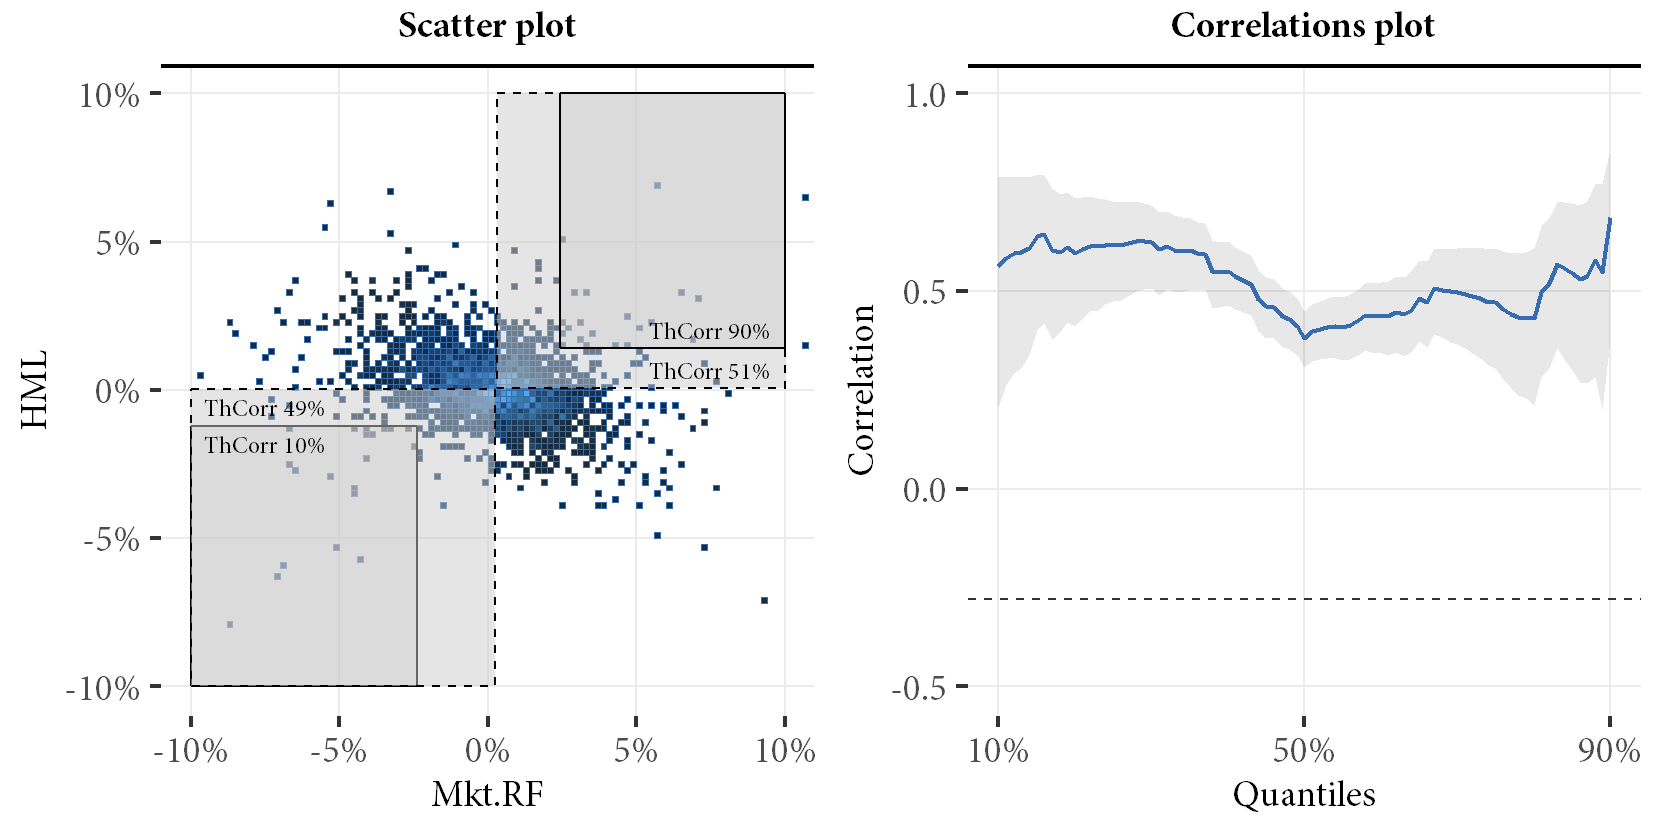
\includegraphics[scale=1]{graphics/threshold_explain_ret.png}  
  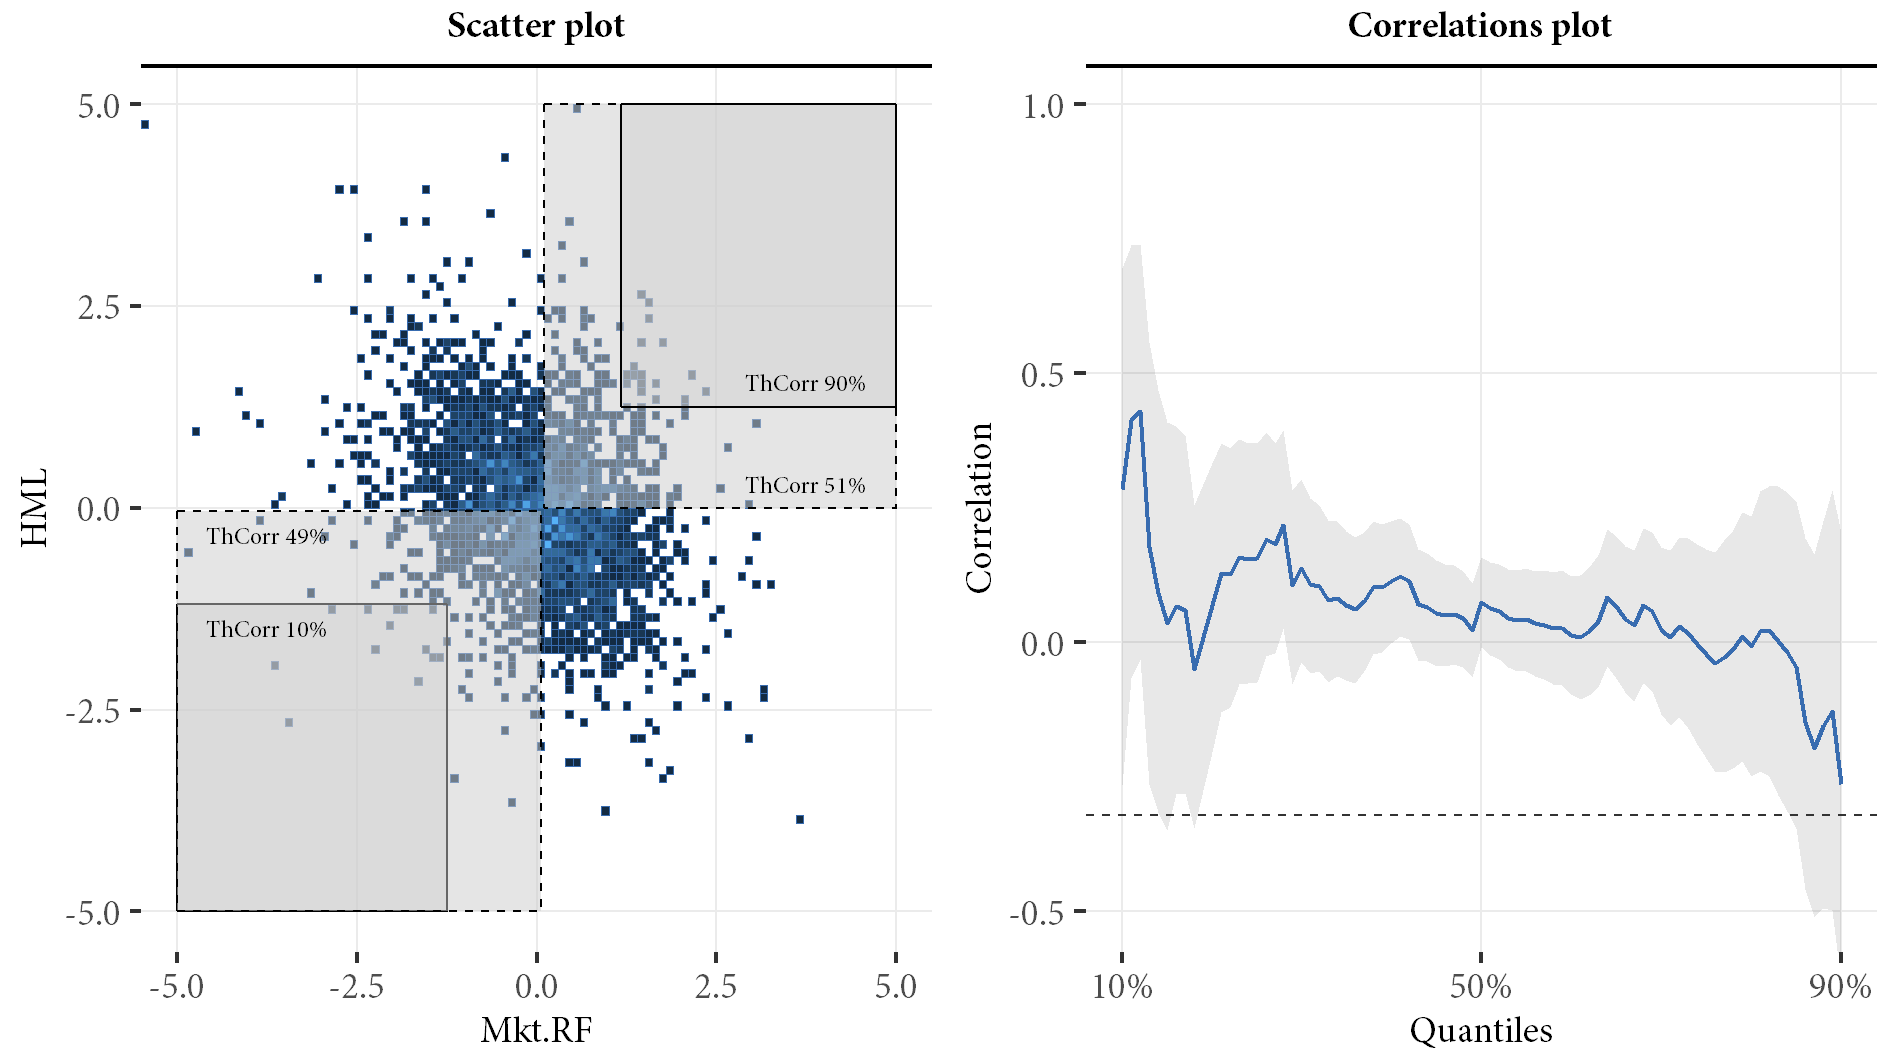
\includegraphics[scale=1]{graphics/threshold_explain_res.png}  
  %\bottomrule
  \vspace{3mm}
  \footnotesize
  Threshold correlation plots with 95\% confidence bounds. Unconditional correlation given by the dashed line. The upper two panels use log return data and the lower two panels use ARMA-GARCH residuals from the chosen models. Weekly data 1963-2016
  \end{minipage}
\end{figure}

In the left hand plots, we see the scatter of returns and ARMA-GARCH residuals of Mkt-RF and HML respectively, and how $p$, found on the x axis of the right hand plot, determines the subset of data that is included in the correlation calculation. Note that the further away from the median we get, the more uncertain the point estimate of the correlation coefficient becomes, as fewer observations are available. For the 49\% and 51\% points, estimates are much more precise as essentially half the data set is available. We also note that the standard correlation, given by the dashed line in the right hand plot, is clearly negative, while threshold correlations in the first and third quadrants are significantly more positive, which shows the usefulness of this analysis; not taking threshold correlations into account provides a vaguer picture of the dependence structure.

Although threshold correlations are nothing but linear correlation coefficients for a subset of the data, they do provide an intuitive measure of tail dependence -- how correlated are returns in bad times? And does this differ from the correlation in good times? Ceteris paribus, assets pairs with weaker or negative threshold correlation as $p \rightarrow 0$ are better diversified, as they have less tendency to coincide in extreme negative realizations. [ADD SOMETHING ABOUT Between two normal distributed variables you expect /\-shape (for positively correlated variables).]

\begin{figure}[H]
  \caption{Threshold correlations on ARMA-GARCH residuals. Page 1/2}
  \label{fig:threshold1}
  %\toprule
  \centering
  \begin{minipage}{\textwidth}
  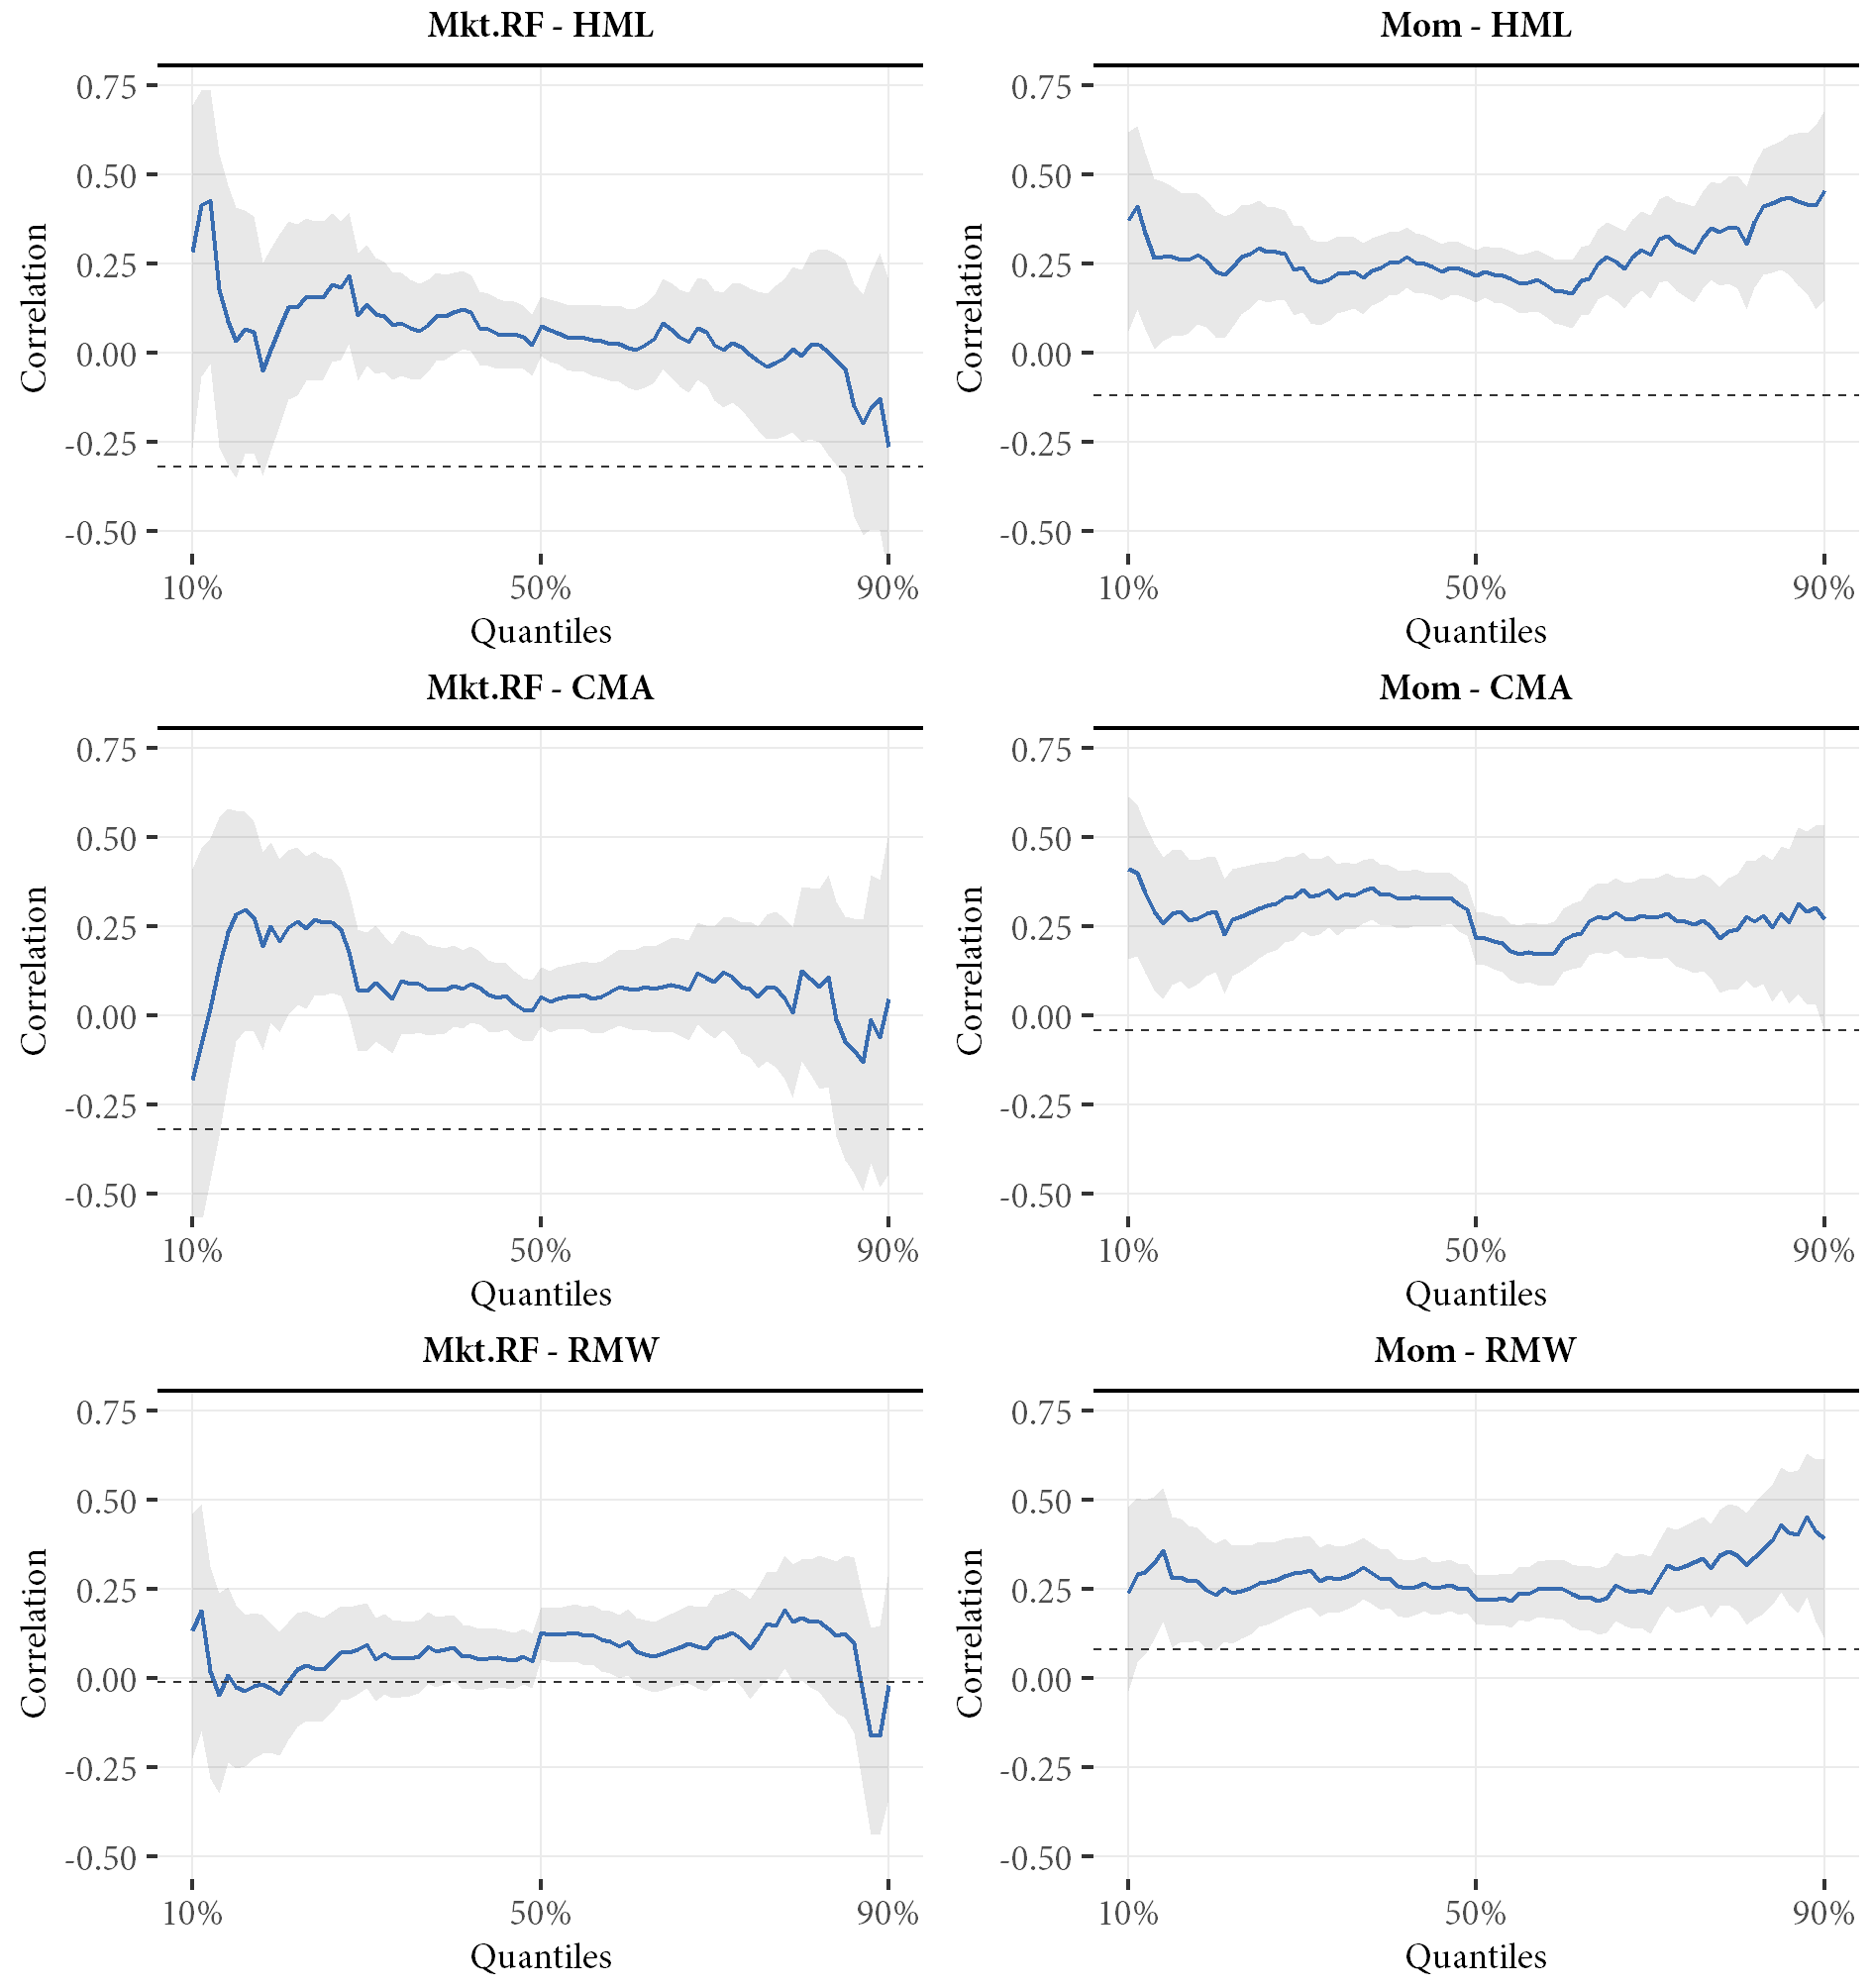
\includegraphics[scale=1]{graphics/threshold1.png}  
  %\bottomrule
  \vspace{3mm}
  \footnotesize
  Threshold correlation plots with 95\% confidence bounds. Correlation pairs in graph titles. Unconditional correlation given by the dashed line. Weekly ARMA-GARCH residuals from the chosen models, all data 1963-2016
  \end{minipage}
\end{figure}
\begin{figure}[H]
  \caption{Threshold correlations on ARMA-GARCH residuals. Page 2/2}
  \label{fig:threshold2}
  %\toprule
  \centering
  \begin{minipage}{\textwidth}
  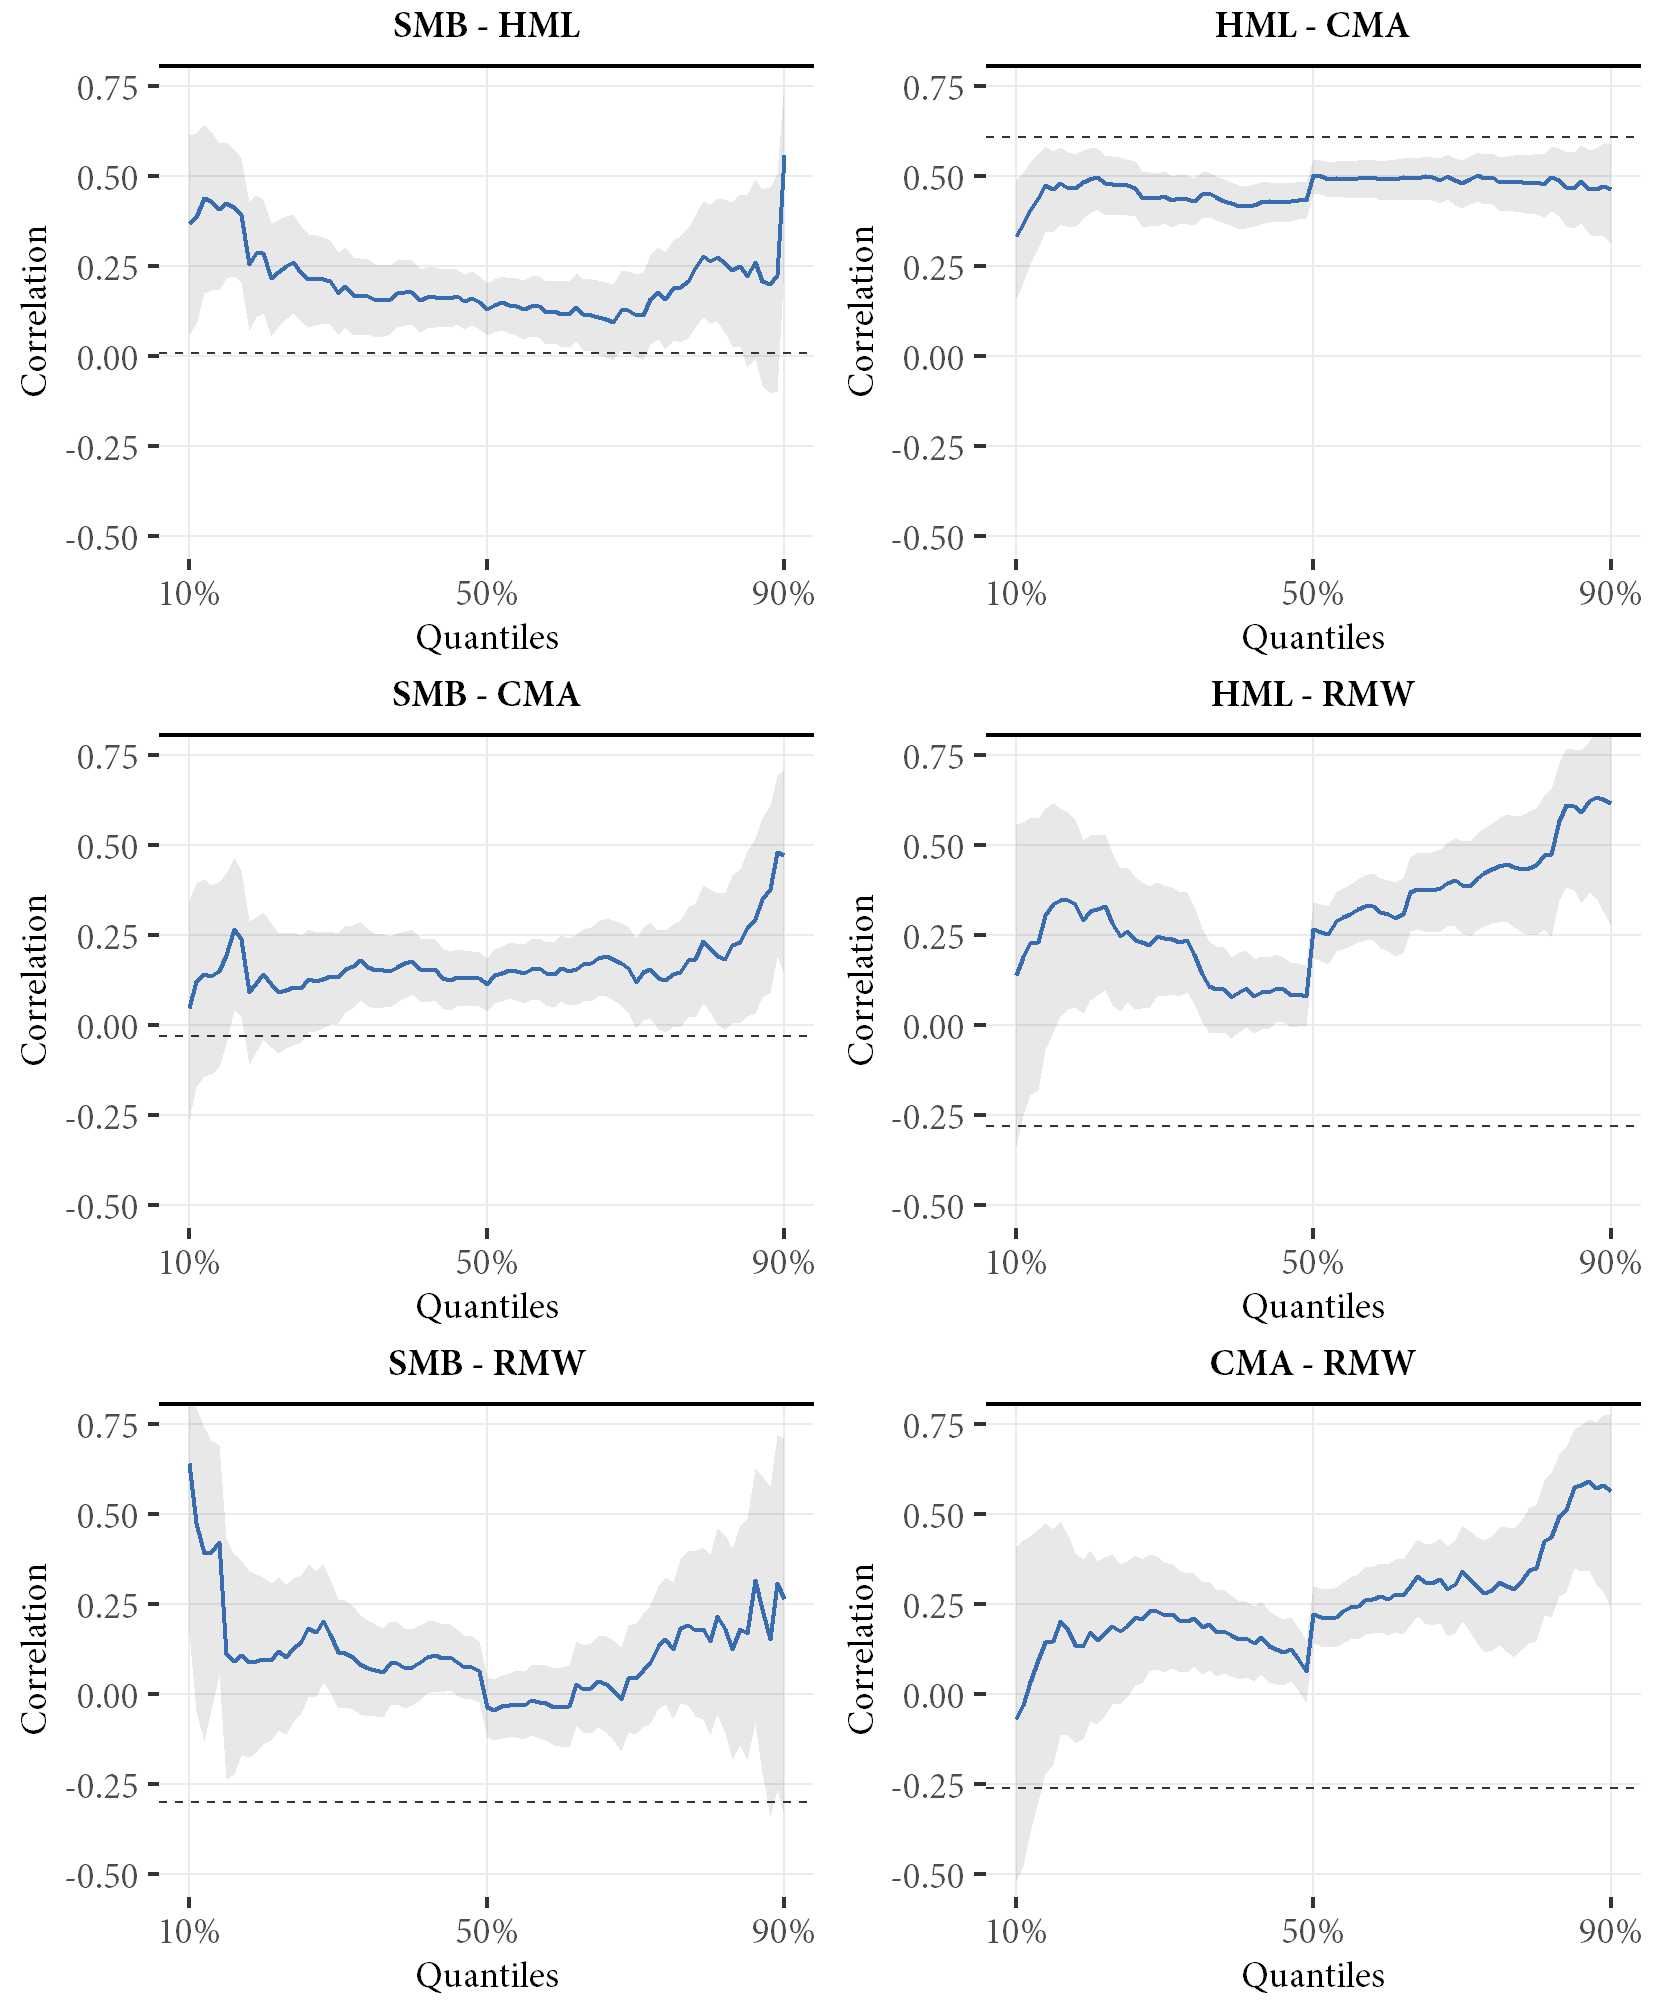
\includegraphics[scale=1]{graphics/threshold2.png}  
  %\bottomrule
  \vspace{3mm}
  \footnotesize
  Threshold correlation plots with 95\% confidence bounds. Correlation pairs in graph titles. Unconditional correlation given by the dashed line. Weekly ARMA-GARCH residuals from the chosen models, all data 1963-2016
  \end{minipage}
\end{figure}

% talk
As previously noted, we use residuals from the ARMA-GARCH models in the threshold correlation analysis instead of returns directly, as the residuals are sanitized of effects that can be explained on the univariate level alone. The plots for the standardized residuals are presented in~\autoref{fig:threshold1} and \autoref{fig:threshold2}. The patterns of returns and residuals are highly similar, with returns exhibiting more extreme patterns (see \autoref{app:threshold_return} for a comparison).

First, we note that the threshold correlation is significantly different from the unconditional correlation coefficient denoted by the dashed line for most factor pairs (with the exception of Mkt-RF - RMW, and CMA - HML). This means that the multivariate dependence of factor strategies has tail dependence that is poorly captured by the standard correlation measure. Conditional on being in the first or third quadrant of returns, assuming a correlation coefficient of the unconditional correlation is misleading. A concrete example is provided by the Mkt-RF and HML pair. In a period when both residuals are observed below their 25\% percentile, the correlation is most certainly not -0.30, but actually positive.

In our multivariate analysis, we would like a model of joint returns to capture this behavior. Risk management is inherently a concern about what happens in the extremes, and the multivariate model should capture some of the tail dependence we observe in threshold correlations.

Second, we note that there is asymmetry around the median for some factor pairs, including the Mom - CMA, RMW - HML, RMW - CMA, and to a lesser extent Mkt-RF - RMW asset pairs. For example, in the Mom-CMA asset pair, the threshold correlation jumps up for the first percentile below the median, indicating that the correlation is higher when both realize below the median than when both realize above the median. This type of asymmetric property, where downside (below the median) correlation is higher than upside correlation is unwanted, as it reflects a poorer diversification in bad times. A good model of joint returns in factor strategies should therefore have flexibility to generate this type of asymmetry.

Third, we note that, although estimated with substantial uncertainty, the threshold correlation do not seem to be constant as $p$ approaches either zero or one. For example, the Mkt-RF - HML asset pair seems to have a downward pattern, where correlation is the most positive in the lowest percentiles of residuals and the most negative in the highest percentile of residuals. In fact, this pattern is unwanted from a diversification perspective, as diversification benefits decrease when the series are realizing in the lowest percentiles.

Fourth, while all other asset pairs exhibit unconditional correlations of around zero or negative, the CMA - HML pair exhibits high and positive correlation of more than 0.60. Furthermore, the threshold correlation estimate is much closer to the unconditional correlation. While all other factor strategy pairs appear to be very good diversifiers, CMA and HML factors look quite similar.

\subsection{Rolling correlation}
\label{subsec:roll_corr}
% method
We compute rolling correlation estimates in order to investigate whether the factor strategies exhibit constant correlation over time. 
\begin{align}
    RCorr(r_{i, t}, r_{j, t})_t^{w} = \frac{\sum^{t}_{t-w+1}(r_{i, t} - \bar{r}_i)(r_{j,t} - \bar{r}_j)}{\sqrt{\sum^{t}_{t-w+1} (r_{i,t} - \bar{r}_i)^2} \sqrt{\sum^{t}_{t-w+1} (r_{j,t} - \bar{r}_j)^2}}
\end{align}
where $r_i$, $r_j$ are the $N \cdot (N-1) / 2$ different pairs of the factor strategies' ARMA-GARCH residuals or log returns and $w$ is the rolling window of data. We use one year of data with $w = 52$ on weekly data. As previously, we use residuals from the ARMA-GARCH models in the rolling correlation analysis instead of returns directly and present results in~\autoref{fig:rolling1} and \autoref{fig:rolling2}.\footnote{A comparison of rolling correlations on returns and residuals is available in~\autoref{app:rolling_return}.}
% plots
\begin{figure}[H]
  \caption{Rolling correlations on ARMA-GARCH residuals. Page 1/2}
  \label{fig:rolling1}
  %\toprule
  \centering
  \begin{minipage}{\textwidth}
  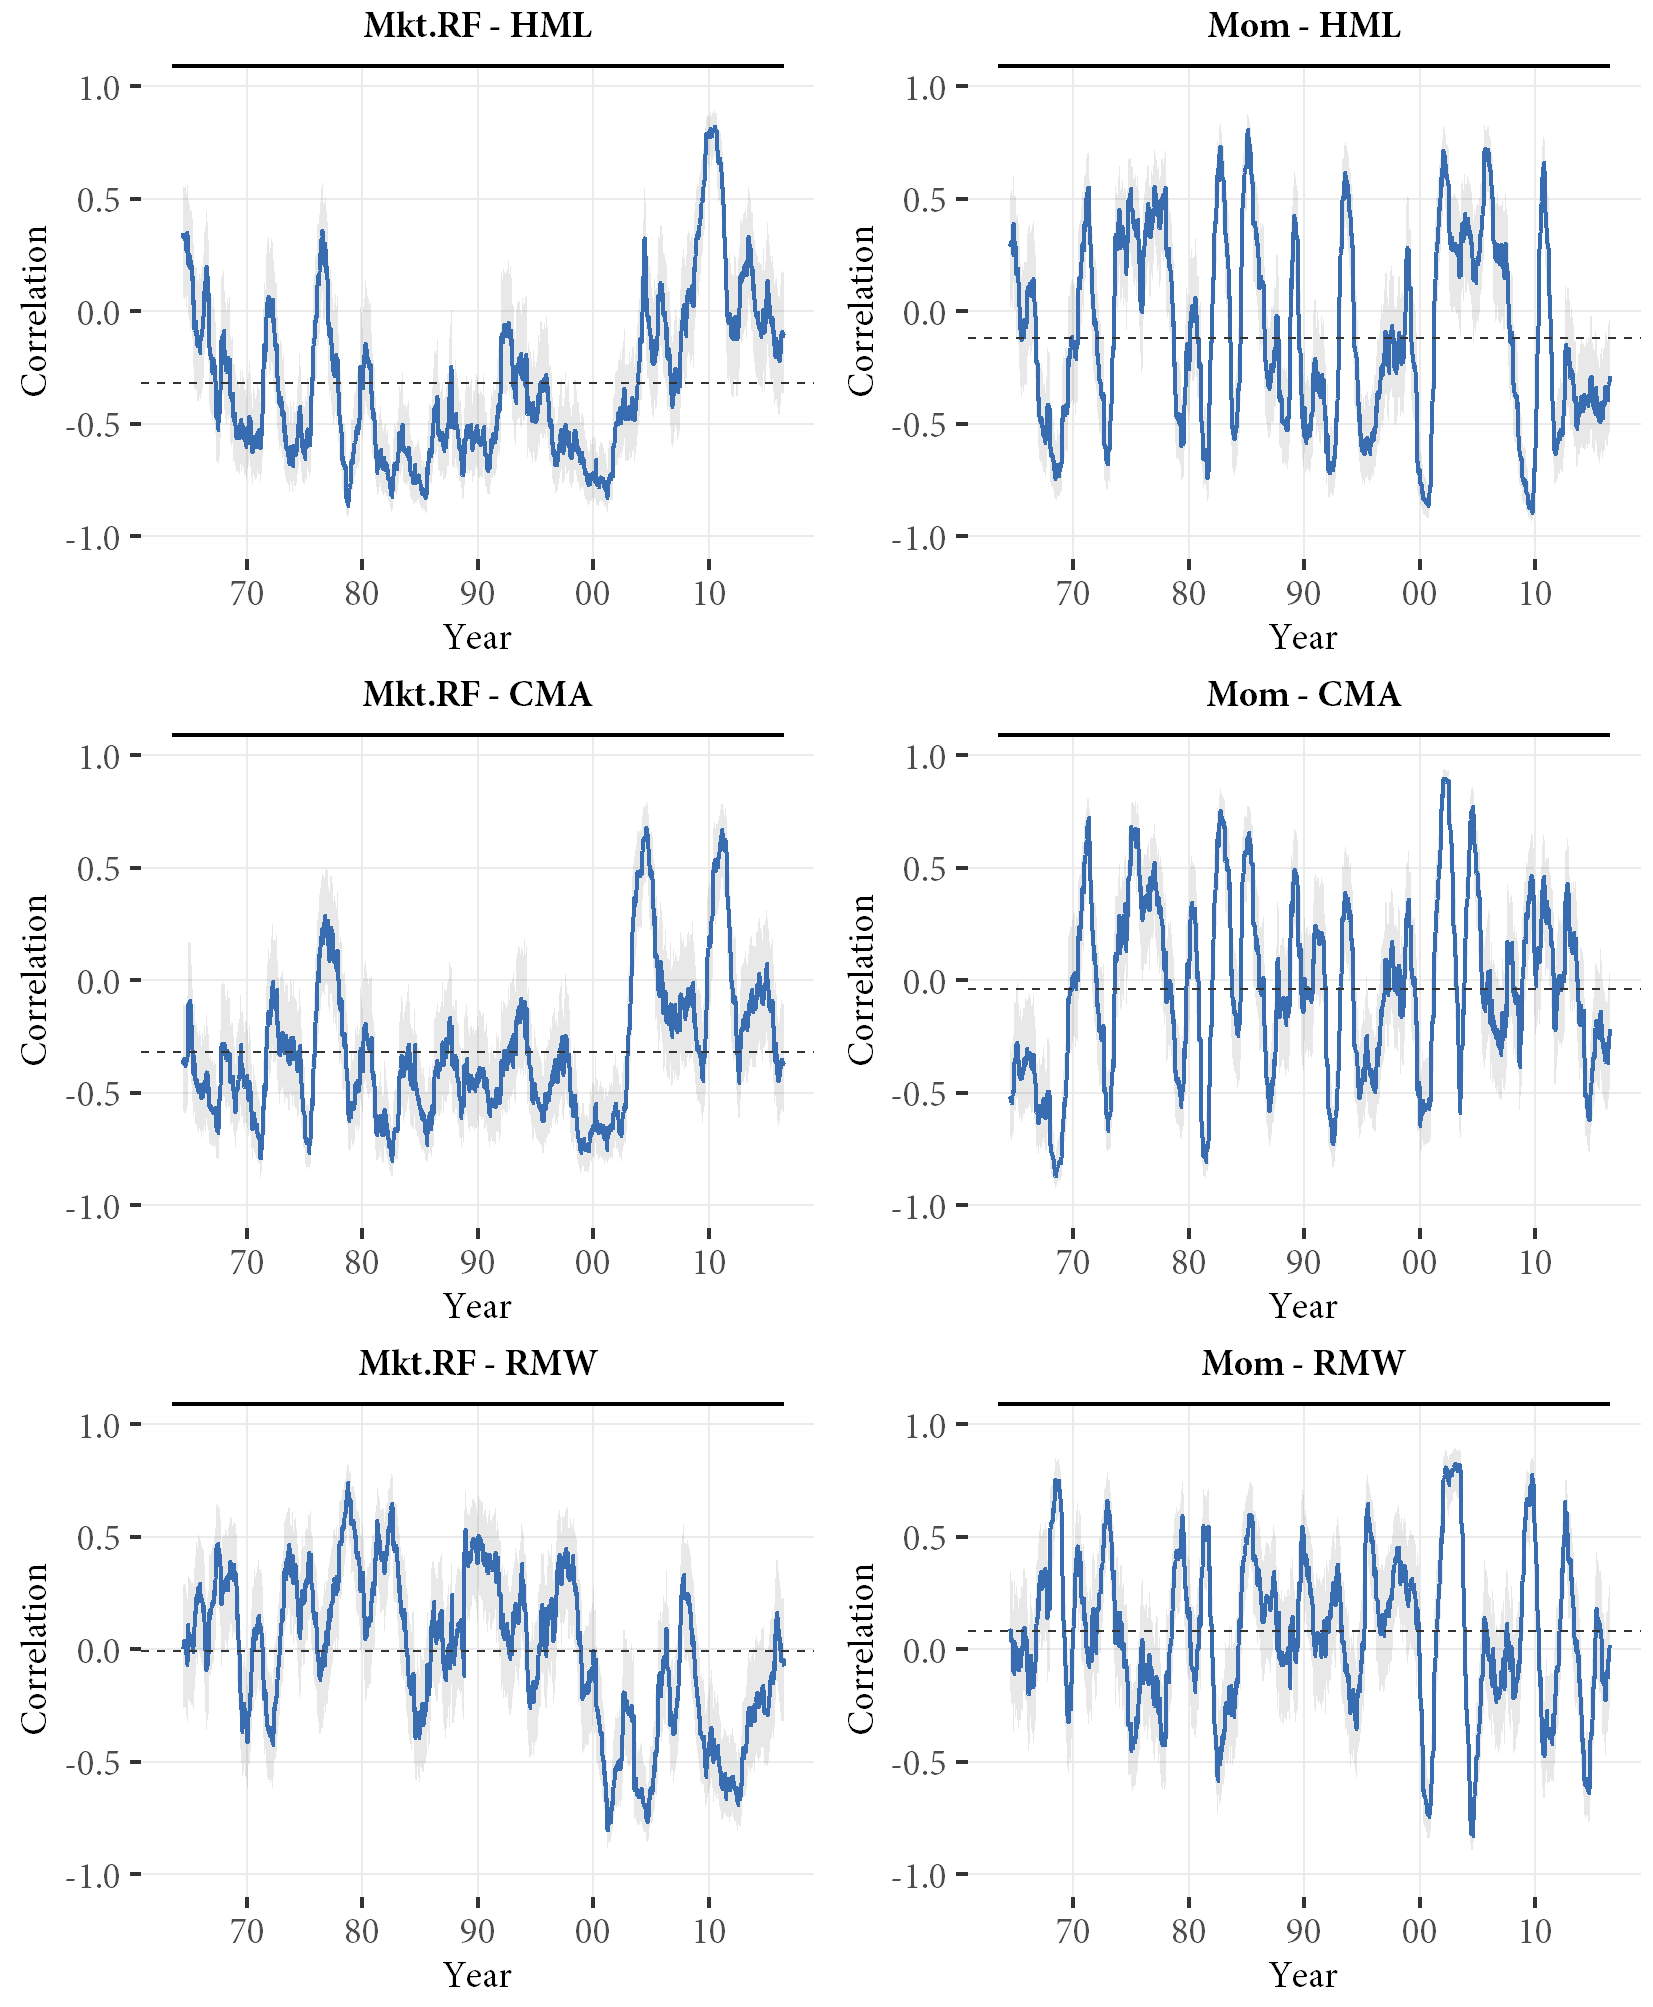
\includegraphics[scale=1]{graphics/rolling1.png}  
  %\bottomrule
  \vspace{3mm}
  \footnotesize
  Rolling correlation plots with 95\% confidence bounds. Correlation pairs in graph titles. Unconditional correlation given by the dashed line. Weekly ARMA-GARCH residuals from the chosen models, all data 1963-2016
  \end{minipage}
\end{figure}
\begin{figure}[H]
  \caption{Rolling correlations on ARMA-GARCH residuals. Page 2/2}
  \label{fig:rolling2}
  %\toprule
  \centering
  \begin{minipage}{\textwidth}
  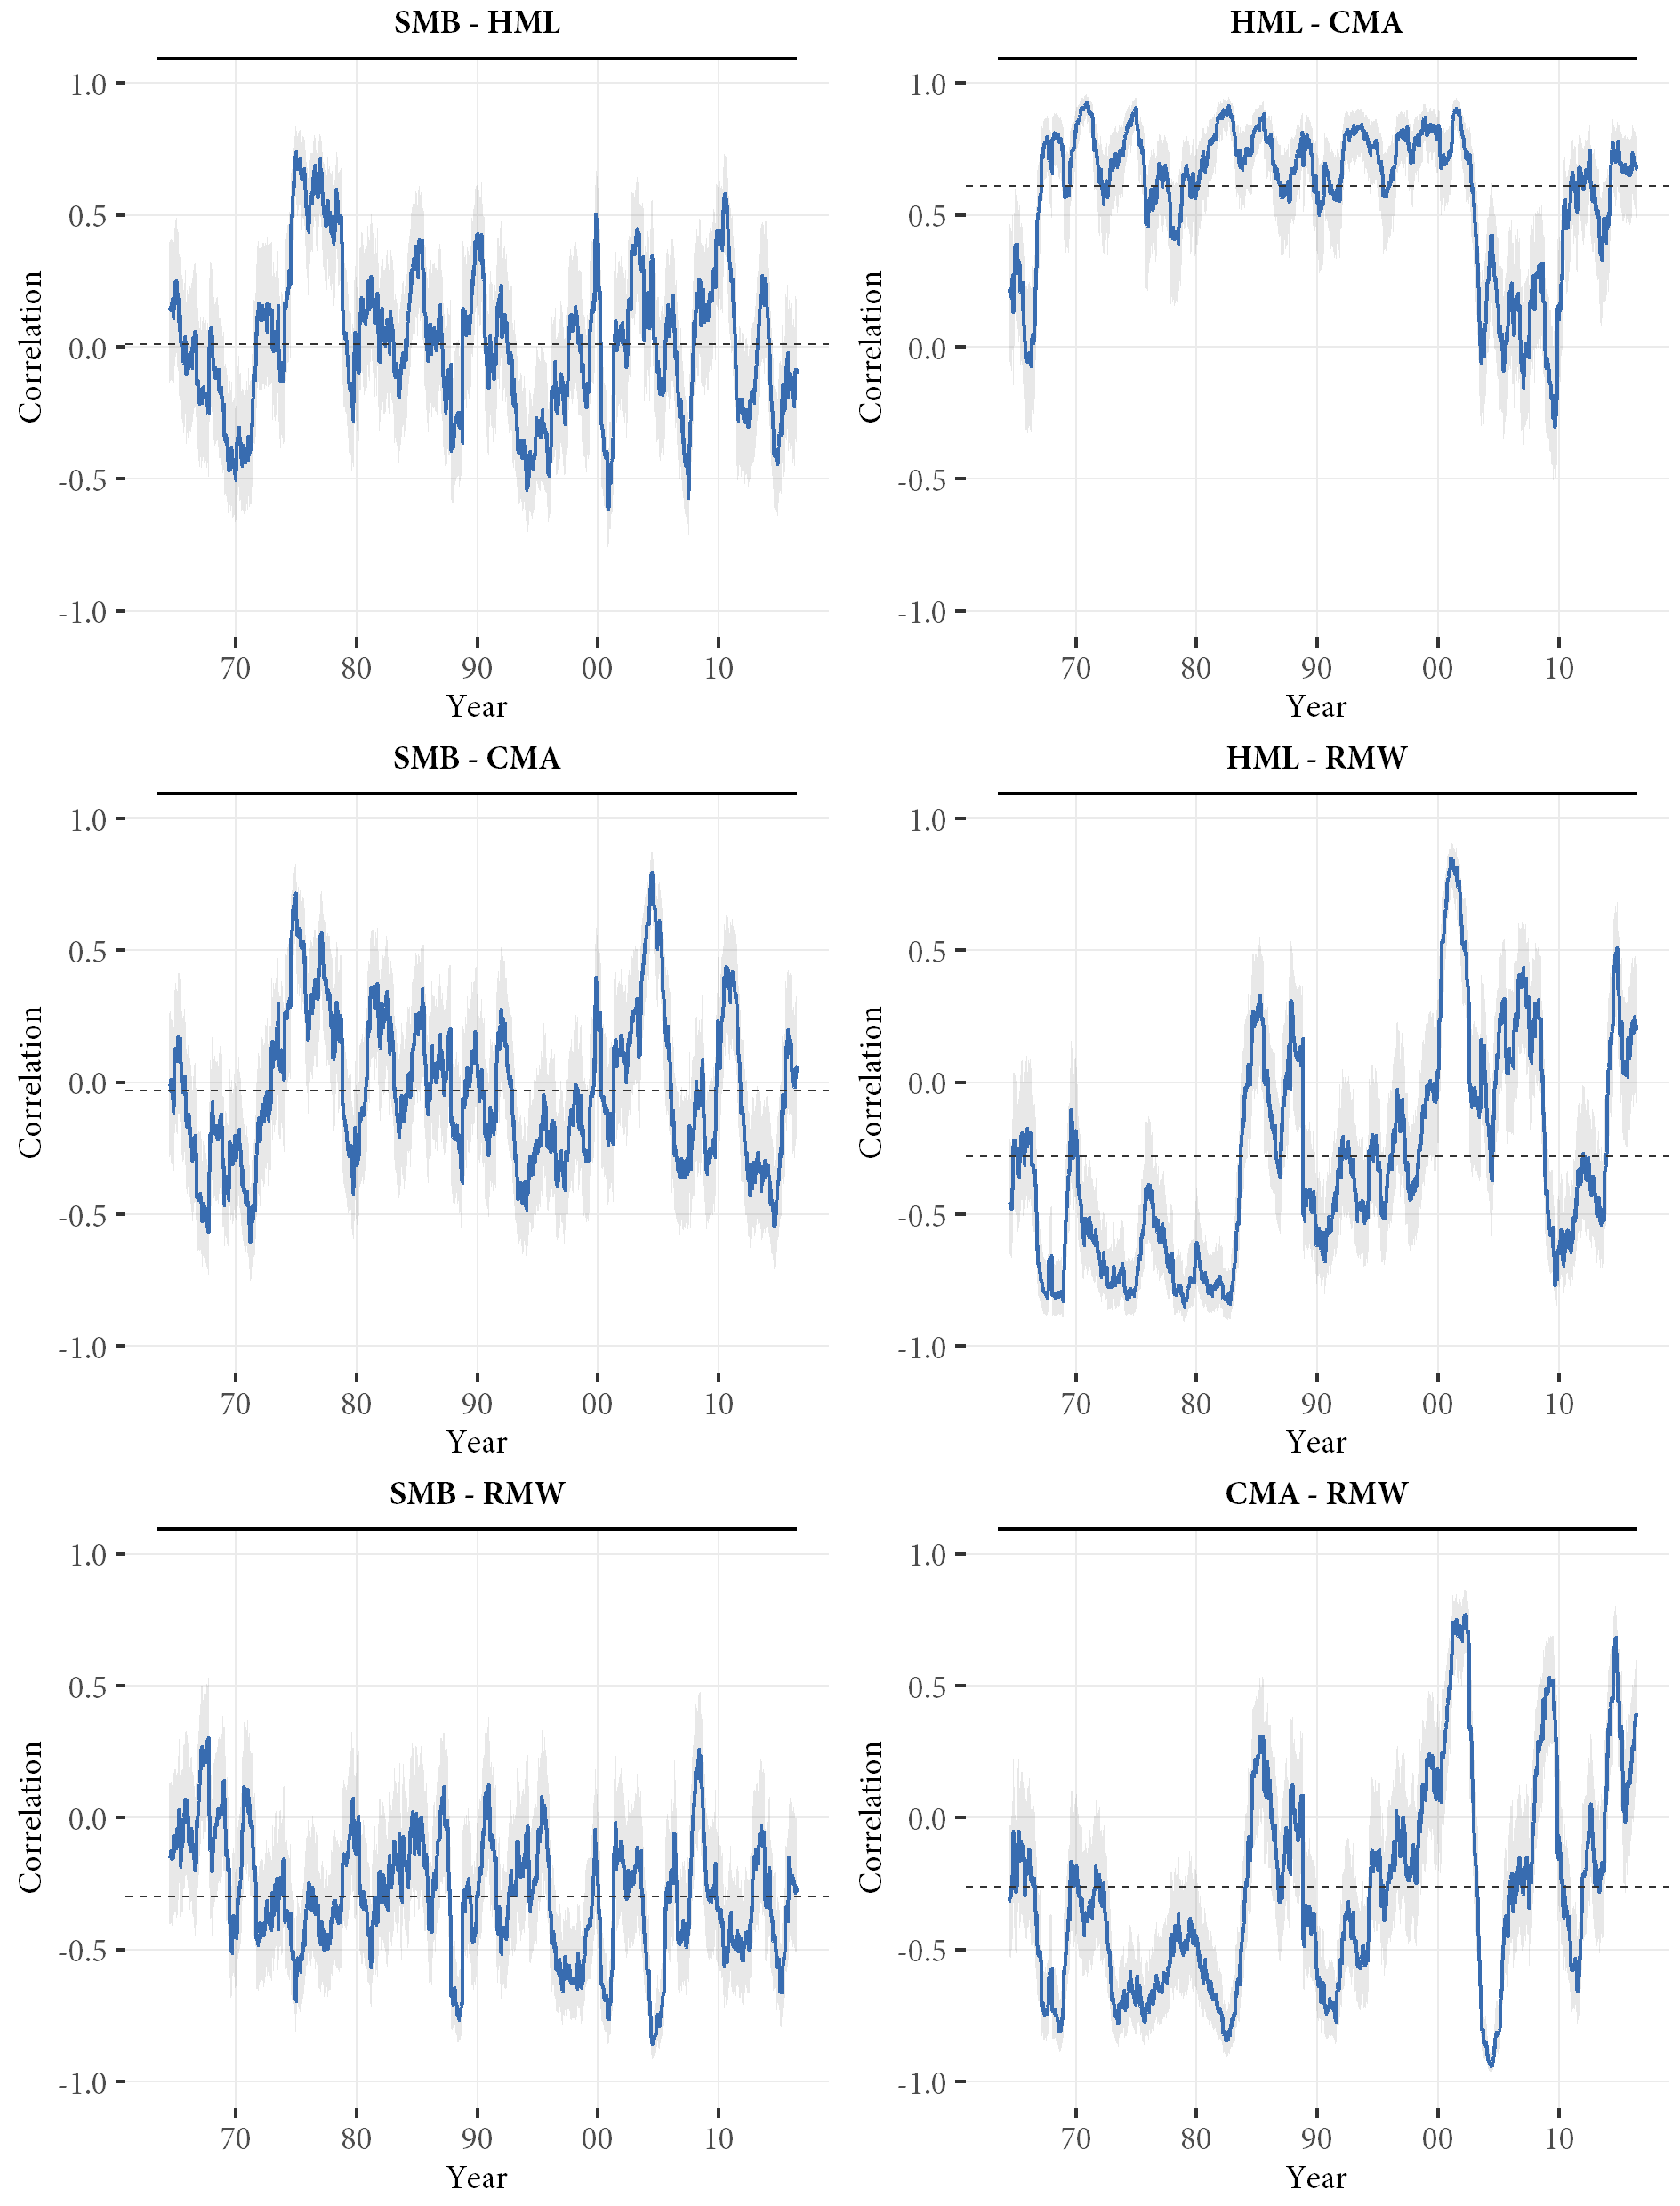
\includegraphics[scale=1]{graphics/rolling2.png}  
  %\bottomrule
  \vspace{3mm}
  \footnotesize
  Rolling correlation plots with 95\% confidence bounds. Correlation pairs in graph titles. Unconditional correlation given by the dashed line. Weekly ARMA-GARCH residuals from the chosen models, all data 1963-2016
  \end{minipage}
\end{figure}
% talk
First, we note that for most factor pairs, the rolling 52-week correlations are highly time-varying. While the unconditional correlation is often around zero, the rolling 52-week correlation ranges between approx. -0.75 and 0.75 for the HML - Mkt-RF factor pair. The time-varying correlations lead us to believe that a suitable model of joint returns will incorporate dynamic correlations. As long as there is some persistence in the series, a dynamic model should have merits in modeling returns jointly, as the best guess of tomorrow's correlation then is not simply the unconditional correlation.

Second, by visual inspection, the correlations of a few asset pairs could be suspected to be non-stationary, either due to overall trending or break points -- for example, the HML - Mkt-RF and CMA - HML asset pairs might have a break point around year 2000, as correlations are higher after this period; and the HML - CMA asset pair might have a break point around the same time, as correlations move outside a relatively close range of 40-90\% to substantially lower levels during 2000-2010. If trends or breakpoints were shown to be present, they could be incorporated in the model of joint returns. We believe that especially the potential upward trend in HML - Mkt-RF and CMA - Mkt-RF is highly interesting, and could mean that diversification benefits of these pairs is becoming weaker, but do not explore this further. In our model, we consider correlations to be stationary.

Third, the HML and CMA factors again stand out as different to other asset pairs. The unconditional correlation is much closer to the rolling estimates than for other factor pairs. However, while the correlation is quite high and constant for much of the early sample period, the lower correlations towards the end give reasons to think that they might in fact provide strong diversification benefits during certain times.

\subsection{Conclusions from analysis of multivariate dependence in univariate residuals}
Univariate residuals appear to be white noise series with no serial correlation or ARCH effects. However, there exists important dependence between residuals of different strategies. First, threshold correlations show that there is tail dependence -- in times when factor pairs simultaneously realize in their best and worst percentiles, correlations are significantly different from the unconditional mean. In fact, threshold correlations are substantially higher than the unconditional mean, which indicates that diversification benefits are smaller than expected when factors simultaneously experience bad times. Second, rolling correlations show that correlations between series are highly time-varying and seem to exhibit persistence. This should mean that a dynamic model of correlations will improve on the description of joint returns.

Both analyses also show that the HML - CMA asset pair is quite different from the other pairs, exhibiting a much higher and more stable dependence. Differently put, they look quite similar as opposed to any other factor pair, and the merit of including both in factor portfolios seems more unclear.

In modeling multivariate dependence, we expect that good candidate models will incorporate both tail dependence and dynamic correlations.
%!TEX root = ../main.tex

\section{Modeling multivariate dependence: Copula Approach} % (fold)
\label{sec:modeling_multivariate_dependence_copula_approach}

\subsection{Multivariate model selection} % (fold)
\label{sub:multivariate_model_selection}

% Dimensionality of MGARCH
Accurate modeling of the joint dynamics of returns is an important and well-studied problem in finance. Unfortunately, straightforward extension of univariate GARCH models to multiple dimensions has proven difficult. Unrestricted multivariate GARCH (MGARCH) models, modeling the conditional covariance matrix directly, become impossible to estimate as the number of covariances grows exponentially with the number of series~\autocite{WhyMGARCHSucks}. It thus becomes necessary to restrict the parameter space, where the BEKK model is a common example~\autocite{BEKKModel}.

% Separate modeling of variance and correlation
A parsimonious solution is to separate the modeling of return and variance dynamics (modeled using ARMA-GARCH) from that of the conditional correlation dynamics. One such approach is encapsulated by the \emph{dynamic conditional correlation} (DCC) model originally proposed by~\autocite{Engle2002} (and its correction \emph{c}DCC by~\autocite{Aielli2013}). The separation allows for consistent (albeit inefficient) two-step estimation. First, univariate GARCH models are estimated on each series (as we do). Second, an autoregressive process for the correlation matrix is fitted to the standardized residuals $\varepsilon_t$ of those models. The separation makes large-scale estimation feasible.

% Asymmetric cDCC
DCC is a useful and tractable model for estimating time-varying correlations between return series. However, as it is a model of correlations only, it cannot capture the asymmetric tail dependency seen in the threshold correlations of residuals. Introducing indicator variables for the strength of correlation, similar to how the leverage effect is captured by GJR-GARCH, is a potential solution (as in the AGDCC model by~\autocite{Cappiello2006}).

% Copula cDCC
Our model for the dependency of factors is the copula version of \emph{c}DCC model called \emph{dynamic asymmetric copula} (DAC), introduced in~\autocite{ChristoffersenErrunzaJacobLanglois2012}. In contrast to fitting the \emph{c}DCC process to standardized residuals directly, we fit a \emph{c}DCC model to a transformation of these shocks. The theoretical motivation behind this transformation is to jointly model returns with separate distributions (e.g. normal and skewed Student's t) in a single framework. The copula approach has the added benefit of separating modeling of the returns themselves from that of the dependency structure.

% subsection multivariate_model_selection (end)

\subsection{Modeling dependence with the DAC model} % (fold)
\label{sub:copula}

% How copula?
Following~\autocite{ChristoffersenErrunzaJacobLanglois2012}, who builds on~\autocite{Patton2006,Sklar1959}, we can decompose the conditional joint density of returns $f_t(r_{1, t+1}, \ldots, r_{N, t+1})$ into the product of a joint copula function $c_t$ of uniform variables $u_{i,t}$ and the marginal univariate distributions $f_{i,t}(r_{i, t+1})$:
\begin{align}
  f_t(r_{1, t+1}, \ldots, r_{N, t+1}) &=
    c_t(u_{1, t+1}, \ldots, u_{N, t+1}) \prod^N_{i = 1}
    f_{i,t}(r_{i, t + 1})
\end{align}
The uniforms $u_{i, t+1}$ are related to the returns by the probability integral transform (PIT):
\begin{align}
  u_{i, t+1} = F_{i,t}(r_{i, t+1}) =
    \int_{-\infty}^{r_{i, t + 1}} f_{i,t}(r_{i, t+1})
\end{align}
In a ARMA-GARCH copula model, the univariate ARMA-GARCH processes describe the conditional densities $f_{i,t}(r_{i, t+1})$, while the copula $c_t$ is a model of the joint behavior of their probability integral transforms. The key benefit of this approach is that $c_t$ is independent of the marginal distributions, which allows separate modeling and estimation. Two-step quasi maximum likelihood, also known as inference-by-margins (IFM) introduced by~\autocite{Joe1997}, first estimates the marginal distributions and subsequently the copula distribution, taking the marginal densities as given. Because the joint density is separate from the marginal densities, we can use different assumptions for each component.

In the most general case, we use a multivariate skewed Student's t DAC model introduced by~\autocite{ChristoffersenErrunzaJacobLanglois2012}. The joint distribution is parametrised by a single degrees of freedom parameter $\nu_c$, $N$ skewness parameters $\gamma_{c,i}$ and a (time-varying) correlation matrix $\Psi_{t}$ (details about the joint density function $c_t$ are in~\autoref{app:ghstmv}). The normal and Student's t copula are nested in this model, as when $\gamma_{c,i}$, we obtain a multivariate Student's t distribution, and if additionally $\nu_c = \infty$, we obtain the multivariate standard normal distribution.

% Interpretation of parameters \gamma, \nu and \Psi?

The copula is made dynamic by evolving the correlation matrix $\Psi_t$ according to an underlying \emph{c}DCC process $Q_t$~\autocites[cf.]{Engle2002,Aielli2013}. Using the notation from~\autocite{ChristoffersenLanglois2013}:
\begin{align}
  Q_t &= (1 - \alpha - \beta) Q
    + \beta Q_{t - 1}
    + \alpha z_{t - 1} z_{t - 1}^\top \\
  \intertext{where $Q_t$ is normalized to the correlation matrix}
  \Psi_t &= Q_t^{-1/2} Q_t Q_t^{-1/2}
\end{align}
The $Q_t$ process is comprised of three components that are weighted according to $\alpha, \beta$: (1) a time-invariant component $Q$, (2) an innovation component from copula shocks $z_{t-1} z_{t-1}^\top$ and (3) an autoregressive component of order one $Q_{t-1}$. In order for the the correlation matrix $\Psi_t$ to be positive definite, $Q_t$ has to be positive definite, which is ascertained by requiring that $\alpha \geq 0$, $\beta \geq 0$ and $(\alpha + \beta) < 1$. The model nests a constant copula by forcing $\alpha = \beta = 0$.

% XXX NOTATION
% XXX cDCC correction for copula shocks

The parameters of the copula model -- the distribution parameters of the multivariate skewed Student's t distribution and the dynamics parameters of the cDCC -- are estimated by maximizing the log-likelihood:
\begin{align}
  \arg\!\max_{\nu_c, \gamma_{ic}, \alpha, \beta} \sum_{t = 1}^T \ln c_t(u_{1, t+1}, \ldots, u_{N, t+1}; \nu_c, \gamma_{ic}, \alpha, \beta)
\end{align}
The process of copula estimation with \emph{c}DCC dynamics is quite involved. A detailed description can be found~\autoref{app:copula_cdcc}.

% subsection copula (end)

% section modeling_multivariate_dependence_copula_approach (end)

%!TEX root = ../main.tex

\section{Multivariate dependence in univariate residuals} % (fold)
%\label
% explain the logic in what we are doing, that there might still be dependence in what looks like white noise residuals
After the univariate modeling of returns in ARMA-GARCH models, we find that the ARMA-GARCH residuals look like white noise, with no serial correlation or ARCH effects. However, when considered jointly, we find that there is substantial dependence remaining in the residual series -- as will be shown in this section, correlation is non-zero and time-varying, and there is tail dependence between the residual series. 

Therefore, we do not use returns directly in the multivariate analysis, as significant parts of the dependence can be removed by univariate models alone. Instead, we use the residuals from the ARMA-GARCH models. The intuition behind this is that we do not want to confuse multivariate dependency in returns with what are in fact just predictable effects that can be understood on the univariate level alone.

Our philosophy, which is in line with the copula methodology, is to try to sanitize the data as far as possible on the univariate level. Then, any dependence left in the residuals can be attributed to multivariate dependence.

\subsection{Threshold correlations}
%\label
% method
Threshold (or exceedance) correlations have previously been used to highlight the asymmetric dependence structure of i.a. country equity indices~\autocite{LonginSolnik2001}, portfolios by industry, size, value and momentum~\autocite{AngChen2002} and factor strategies~\autocite{ChristoffersenLanglois2013}. The following analysis is still new as it adds the factors investment (CMA) and profitability (RMW). We follow~\textcite{ChristoffersenLanglois2013} definition of threshold correlation
\begin{align}
    ThCorr(r_i, r_j) = 
    \begin{cases} 
        Corr\Big(r_i, r_j \,|\, r_i < F_i^{-1}(p), r_j < F_j^{-1}(p)\Big)  & \text{for } p < 0.5 \\
        Corr\Big(r_i, r_j \,|\, r_i \geq F_i^{-1}(p), r_j \geq F_j^{-1}(p)\Big)  & \text{for } p \geq 0.5
    \end{cases}
\end{align}
where $F_i^{-1}(p)$ the empirical quantile of $r_i$ at percentile $p$. 

Graphically, threshold correlation are understood as the standard correlation estimate in more and more distant parts of the first and third quadrant as $p$ approaches either zero or unity. This subsetting of data is illustrated in \autoref{fig:illustrate_threshold}. 

On the left hand plot, we see the scatter of returns on Mkt-RF and HML, and how $p$, found on the x axis of the right hand plot, determines the subset of data that is included in the correlation calculation. Note that the further away from the median we get, the more uncertain the point estimate of the correlation coefficient becomes, as fewer observations are available. For the 49\% and 51\% points, estimates are much more precise as essentially half the data set is available. We also note that the standard correlation, given by the dashed line in the right hand plot, is clearly negative, while threshold correlations in the first and third quadrants are significantly more positive, which shows the usefulness of this analysis; not taking threshold correlations into account provides a vaguer picture of the dependence structure.

Although threshold correlations are nothing but linear correlation coefficients for a subset of the data, they do provide an intuitive measure of tail dependence -- how correlated are returns in bad times? And does this differ from the correlation in good times? Ceteris paribus, assets pairs with weaker or negative threshold correlation as $p \rightarrow 0$ are better diversified, as they have less tendency to coincide in extreme negative realizations.

% plots [possibly add diff series/residuals]
As previously noted, we use residuals from the ARMA-GARCH models in the threshold correlation analysis instead of returns directly. The plots for the standardized residuals are presented in~\autoref{fig:threshold_corr1, threshold_corr2} The patterns of returns and residuals are highly similar, with returns exhibiting more extreme patterns (see \autoref{app:threshold_returns1, app:threshold_return2} for a comparison).

% talk


\subsection{Rolling correlation}
%\label
%method
We compute rolling correlation estimates in order to investigate whether the factor equity strategies exhibit constant correlation over time. 
\begin{align}
    RCorr(r_{i, t}, r_{j, t})_t^{w} = \frac{\sum^{t}_{t-w+1}(r_{i, t} - \bar{r}_i)(r_{j,t} - \bar{r}_j)}{\sqrt{\sum^{t}_{t-w+1} (r_{i,t} - \bar{r}_i)^2} \sqrt{\sum^{t}_{t-w+1} (r_{j,t} - \bar{r}_j)^2}}
\end{align}
where $r_i$, $r_j$ are the $N \cdot (N-1) / 2$ different pairs of the factor strategies' log returns and $w$ is the rolling window of data. We use one year of data with $w = 52$ on weekly data.
%plots, talk


\section{Modeling multivariate dependence: Copula} % (fold)
%\label


\subsection{Multivariate model selection}
%\label
% why copula?
% explain logic and intuition: this is a parsimonious way, and solves the two issues with asymmetry and time-variation to some extent
% other models BEKK, etc have issues with dimensionality or can't capture the features of threshold and rolling

\subsection{Copula}
%\label
% method of model
% estimation of model

\subsection{Copula results with constant correlations}
%\label
% diagnostics of fit
% include threshold correlations, look better for skewed t, gaussian bad
\subsection{Copula results}
% TABLES NEED TO BE MODIFIED IN THE FOLLOWING WAYS
% 1) Change {tabular} to {tabularx}{\textwidth} and make leftmost column an X column
%     and change top and bottom \hline to \toprule \bottomrule
%
% paste the following at start but before & \multicolumn
%
% \begin{tabularx}{\textwidth}{@{\extracolsep{5pt}} X D{.}{.}{-3} D{.}{.}{-3} D{.}{.}{-3} } 
% \\[-1.8ex] \midrule
% \\[-1.8ex] 
%
% paste the following at end after R2 row but before Note row
% \bottomrule \\[-1.8ex] 
%
% 2) Change the variable names to greeks
% 3) Change specification names if needed
% 4) Change R2 to LLH and add similar lines for Ljung-Box and ARCH-LM
% 5) Add label and caption
% 6) Paste this to get table heading description
% 7) Copy table heading tabularx footnote size text
%
% \begin{tabularx}{\textwidth}{X}
% \\[-1.8ex]\toprule
%\\[-1.8ex] 
% text goes here
% \end{tabularx}
%
% 6) Copy the whole table, only change caption, label, factor/spec labels and (1)-(3) to (4)-(6)
% Table created by stargazer v.5.2 by Marek Hlavac, Harvard University. E-mail: hlavac at fas.harvard.edu
% Date and time: ons, okt 12, 2016 - 12:37:02
% Requires LaTeX packages: dcolumn 
\begin{table}[!htbp] \centering 
  \caption{Copula results: Constant specifications} 
  \label{tab:copula_estimates_constant} 
\begin{tabularx}{\textwidth}{X}
  \\[-1.8ex]\toprule
  \\[-1.8ex] 
  \footnotesize Parameter estimates from constant copula models based on uniform residuals from ARMA-GARCH models. Stationary bootstrap standard errors in parentheses, following \textcite{PolitisRomano1994}. Copula parameters: $\nu$ is the degree of freedom, $\gamma$ is the vector of skewness parameters, $\alpha, \beta$ are the shock loading and autoregressive loading of the \textit{c}DCC process. All data 1963-07-05 - 2016-07-01. 
\end{tabularx}
\begin{tabularx}{\textwidth}{@{\extracolsep{5pt}} X D{.}{.}{-3} D{.}{.}{-3} D{.}{.}{-3} } 
  \\[-1.8ex]\midrule
  \\[-1.8ex] 
   & \multicolumn{3}{c}{Constant copula models} \\ 
  \cline{2-4} 
  \\[-1.8ex] & \multicolumn{1}{c}{(1)} & \multicolumn{1}{c}{(2)} & \multicolumn{1}{c}{(3)}\\ 
  \\[-1.8ex] & \multicolumn{1}{c}{Gaussian} & \multicolumn{1}{c}{Student-\textit{t}} & \multicolumn{1}{c}{Skewed Student-\textit{t}}\\ 
  \hline \\[-1.8ex] 
 $\nu$ &  & 6.625 & 6.671 \\ 
  &  & () & () \\ 
  & & & \\ 
 $\gamma_{Mkt.RF}$ &  &  & -0.057 \\ 
  &  &  & () \\ 
  & & & \\ 
 $\gamma_{SMB}$ &  &  & -0.103 \\ 
  &  &  & () \\ 
  & & & \\ 
 $\gamma_{Mom}$ &  &  & -0.202 \\ 
  &  &  & () \\ 
  & & & \\ 
 $\gamma_{HML}$ &  &  & 0.103 \\ 
  &  &  & () \\ 
  & & & \\ 
 $\gamma_{CMA}$ &  &  & 0.076 \\ 
  &  &  & () \\ 
  & & & \\ 
 $\gamma_{RMW}$ &  &  & 0.021 \\ 
  &  &  & () \\ 
  & & & \\ 
\hline \\[-1.8ex] 
Observations & \multicolumn{1}{c}{2,766} & \multicolumn{1}{c}{2,766} & \multicolumn{1}{c}{2,766} \\ 
LLH & \multicolumn{1}{c}{1,169} & \multicolumn{1}{c}{1,556} & \multicolumn{1}{c}{1,573} \\ 
No. parameters & \multicolumn{1}{c}{15} & \multicolumn{1}{c}{16} & \multicolumn{1}{c}{22} \\ 
BIC & \multicolumn{1}{c}{-2,220} & \multicolumn{1}{c}{-2,985} & \multicolumn{1}{c}{-2,971} \\ 
Correlation $(Q)$ persistence $(\alpha+\beta)$ & \multicolumn{1}{c}{N/A} & \multicolumn{1}{c}{N/A} & \multicolumn{1}{c}{N/A} \\ 
\bottomrule \\[-1.8ex] 
\textit{Note:}  & \multicolumn{3}{c}{$^{*}$p$<$0.1; $^{**}$p$<$0.05; $^{***}$p$<$0.01} \\ 
\end{tabularx} 
\end{table} 


\subsection{Copula results with dynamic correlations}
%\label
% still haven't captured dynamic, lets do this now
% diagnostics of fit
% why we prefer symmetric t
% correlation patterns over time in-sample graph looks very much like the data rolling
% Table created by stargazer v.5.2 by Marek Hlavac, Harvard University. E-mail: hlavac at fas.harvard.edu
% Date and time: ons, okt 12, 2016 - 12:37:02
% Requires LaTeX packages: dcolumn 
\begin{table}[!htbp] \centering 
  \caption{Copula results: \textit{c}DCC specifications} 
  \label{tab:copula_estimates_dynamic} 
\begin{tabularx}{\textwidth}{X}
\\[-1.8ex]\toprule
\\[-1.8ex] 
\footnotesize Parameter estimates from dynamic copula models based on uniform residuals from ARMA-GARCH models. Stationary bootstrap standard errors in parentheses, following \textcite{PolitisRomano1994}. Copula parameters: $\nu$ is the degree of freedom, $\gamma$ is the vector of skewness parameters, $\alpha, \beta$ are the shock loading and autoregressive loading of the \textit{c}DCC process. All data 1963-07-05 - 2016-07-01. 
\end{tabularx}
\begin{tabularx}{\textwidth}{@{\extracolsep{5pt}} X D{.}{.}{-3} D{.}{.}{-3} D{.}{.}{-3} } 
\\[-1.8ex]\midrule
\\[-1.8ex] 
 & \multicolumn{3}{c}{Dynamic copula models} \\ 
\cline{2-4} 
\\[-1.8ex] & \multicolumn{1}{c}{(4)} & \multicolumn{1}{c}{(5)} & \multicolumn{1}{c}{(6)}\\ 
\\[-1.8ex] & \multicolumn{1}{c}{Gaussian} & \multicolumn{1}{c}{Student-\textit{t}} & \multicolumn{1}{c}{Skewed Student-\textit{t}}\\ 
\hline \\[-1.8ex] 
 $\nu$ &  & 11.936 & 11.881^{***} \\ 
  &  & () & (1.064) \\ 
  & & & \\ 
 $\gamma_{Mkt.RF}$ &  &  & -0.078 \\ 
  &  &  & (0.054) \\ 
  & & & \\ 
 $\gamma_{SMB}$ &  &  & -0.175^{**} \\ 
  &  &  & (0.077) \\ 
  & & & \\ 
 $\gamma_{Mom}$ &  &  & -0.145^{*} \\ 
  &  &  & (0.073) \\ 
  & & & \\ 
 $\gamma_{HML}$ &  &  & 0.083 \\ 
  &  &  & (0.058) \\ 
  & & & \\   
 $\gamma_{CMA}$ &  &  & 0.001 \\ 
  &  &  & (0.063) \\ 
  & & & \\ 
 $\gamma_{RMW}$ &  &  & 0.095 \\ 
  &  &  & (0.061) \\ 
  & & & \\ 
 $\alpha$ & 0.065 & 0.068 & 0.068^{***} \\ 
  & () & () & (0.007) \\ 
  & & & \\ 
 $\beta$ & 0.915 & 0.913 & 0.913^{***} \\ 
  & () & () & (0.011) \\ 
  & & & \\ 
\hline \\[-1.8ex] 
Observations & \multicolumn{1}{c}{2,766} & \multicolumn{1}{c}{2,766} & \multicolumn{1}{c}{2,766} \\ 
LLH & \multicolumn{1}{c}{2,791} & \multicolumn{1}{c}{2,978} & \multicolumn{1}{c}{2,989} \\ 
No. parameters & \multicolumn{1}{c}{17} & \multicolumn{1}{c}{18} & \multicolumn{1}{c}{24} \\ 
BIC & \multicolumn{1}{c}{-5,447} & \multicolumn{1}{c}{-5,813} & \multicolumn{1}{c}{-5,788} \\ 
Correlation $(Q)$ persistence $(\alpha+\beta)$ & \multicolumn{1}{c}{0.981} & \multicolumn{1}{c}{0.981} & \multicolumn{1}{c}{0.981} \\ 
\bottomrule \\[-1.8ex] 
\textit{Note:}  & \multicolumn{3}{c}{$^{*}$p$<$0.1; $^{**}$p$<$0.05; $^{***}$p$<$0.01} \\ 
\end{tabularx} 
\end{table} 
% potentially subsection exogenous regressors
%

\section{Putting the model to work}
%\label
% now, lets see what this model can say about a few things

\subsection{Mean-variance investing}
%\label
% fama french regressions, what actually happens to MV weights, do they go to zero?
% explain method for out-of-sample distributions, simulation based
% show that weights don't go to zero, not for sample and not for advanced super copula model
% what is the out-of-sample investment performance of relying on the best copula model?
% it looks pretty good but not drastically better than relying on sample average - OOS is hard

\subsection{Conditional diversification benefits}
%\label
% what are the theoretical diversificaiton benefits of including hml? is HML or CMA riskier if one can only choose either or? CDB analysis

\pagebreak
%!TEX root = ../main.tex

\section{Discussion and conclusion} % (fold)
\label{sec:discussion_conclusion}

The first key finding of this thesis is that the classic value factor, HML, is still highly relevant for factor investors. 

Zero-cost regressions in the five-factor model suggest that HML may be fully explained by the remaining four factors, but we find evidence to the contrary. The actual implementation of mean-variance optimizations under the only constraint of non-negative weights gives a positive allocation to the HML factor. First, we have shown this using constant sample estimators as inputs in the mean-variance model on data 1963--2016. The sceptic reader will, however, object to the conclusion based on sample data alone, as a model is never better than its inputs; and sample estimates do not give a sense of optimal weights over time.

We show that, in our data, there is clear evidence of non-normality and time-variation in the dependency across factors. A mean-variance optimization that is run solely on the basis of sample estimates will ignore these features of the data, and the positive allocation to HML might be an uninteresting solution to the optimization problem.

To mitigate these concerns, we also run the mean-variance optimization using dynamic inputs from a copula model, which can generate a conditional distribution of returns that captures both the non-normality and the time-variation in dependency. Under such inputs, the allocation to HML is even greater, indicating that the classic value factor is even more attractive than sample inputs suggest.

Although variance is the staple measure of risk, we also investigate whether risk beyond the first two moments can provide reasons against the HML factor. The copula model has allowed us to infer the full distribution of returns, and we shift our focus to the tail of the distribution. Here, we find that the diversification benefit of HML is at least as great, if not greater, than that of CMA. HML can by no means be considered a worse diversifier against tail risk, as measured by expected shortfall, than CMA.

We believe that the reason why zero-cost regressions indicate that HML does not add value is that the regressions are misspecified. The omission of an important sixth factor strategy, momentum, creates a bias on all the factor loadings, and leads to not recognizing the added value of HML. While the role of HML as a unique addition was already defended by \textcite{Asness2015}, we have pursued the argument and can conclude that optimizations lead to positive allocations to the HML strategy.

Our second key finding is that HML is highly similar, but not quite the same as CMA. On a closer look, differences emerge, and we believe that factor investors should combine both factors with consideration.

There is important theoretical and empirical support for a overlap in the stock positions that comprise HML and CMA, which results in a substantially higher correlation for this factor pair than for any other factor pair. The dependence between the two factors is also more stable, and does not exhibit the same pattern of tail dependece as do other factor pairs. 

Still, one factor cannot replace the other -- they do exhibit different properties, as HML firms are more profitable and exhibit less momentum, and generate return premia that mean-variance optimization suggests combining. Beyond the risk-reward of the first two moments, analysis of the full return distribution from the copula model shows that the diversification benefit of adding either HML or CMA to a portfolio is not constant over time. Sometimes HML is the better diversifier, sometimes CMA is better, but no pattern emerges as to which factor is better than the other. We see no reason for investors to choose either one or the other, as both provide valuable diversification, and even better, they do so at different times.

However, we strongly believe that investors should consider the two factors jointly when building portfolios: When one of the two factors is included to a factor portfolio already containing the second, the first factor almost exclusively cannabilizes on the weight from the second. Our findings support the existing theoretical and empirical evidence of an overlap in the firms that comprise the two strategies. All in all, we are wary of factor weighting schemes that suggest pure equal-weights for HML and CMA. While such schemes are valuable for factor investing in general, as they avoid the pitfall of factor (mis)timing, they should be designed in a manner that takes the close link between HML and CMA into account. This pair has a very different dependence from all other pairs -- and so should also the allocation policy be different.

A third finding of this thesis is the strength of the profitability factor. The factor covaries negatively with most factors and receives zero or negative factor loadings in zero-cost regressions. The exclusion of RMW in our diversification benefit analysis completely pulls the plug on diversification, making periods of low diversification both more frequent and much more severe. Furthermore, the factor receives high allocations both using sample and model inputs in the mean-variance framework. The fact that there are no strong explanations of the profitability factor as a risk premium makes these findings even more puzzling: While investing in quality firms is by no means a new notion, there are always two investors to every trade, and the reasons for not holding profitable firms are unclear. Our takeaway is that all funds and investors in the factor space should seriously consider adding this new factor.

During the writing of this thesis, we also considered studying additional emerging factors, in particular the low volatility and betting against beta factors. At a first glance, we found highly diversifying characteristics of these factors, which remind us of RMW. It would be especially interesting to study their impact on tail risk, following the conditional diverisfication benefit analysis. We did in the end not include them as we hone in on the discussion regarding HML's role in the five- and six-factor models.

A substantial part of this thesis is built upon a rather opaque and involved copula model. While we are generally comfortable with the estimation procedure and robustness of the model, we acknowledge that it does lack the power to properly explain asymmetries in tail dependence. A natural route for an extension to a more flexible methodology would be to consider vine copulas in place of the multivariate copula we use. We also believe that the advances of regime switching models could prove fruitful in the factor setting, as such models can more rapidly adjust to shocks.

In unreported results, we have also studied out-of-sample investing with factor timing based on the copula model, but find results to be lackluster. While the copula model can ex post shed light on the roles of different factors, it is not useful for a priori portfolio allocation. This is, however, highly coherent with the preference of money managers to use static weights.\footnote{See i.a. \textcite{AQRSiren}, \textcite{BlackRock}, \textcite{MSCI} and \textcite{Robeco}.} Out-of-sample factor timing is hard, and please note that we do not purport to create a model for investment uses -- our contribution is only possible ex-post. While MV and CDB analysis based on dynamic weights may seem counter-intuitive at first, as investors use static weights, we argue that the dynamic analysis is a powerful tool for evaluation purposes.
\pagebreak
\printbibliography
\pagebreak
%!TEX root = ../main.tex
\appendix
\appendixpageoff
\section{Appendix A. Skewed Student-\textit{t} distribution} \label{App:AppendixA}
In line with stylized facts on financial return series, the factor strategies exhibit fat tails and skewness - features that are poorly represented by the normal Gaussian. Our univariate estimations as well as our copula builds on the~\textcite{Hansen1994} skewed Student-\textit{t} distribution. The skewed Student-\textit{t} distribution is, more generally, nested in the generalized hyperbolic distribution~\autocite{McNeilFreyEmbrecht2005}.

The random vector X is distributed multivariate generalized hyperbolic if
\begin{align}
    X \sim \mu + \sqrt{W} A Z + \gamma W
\end{align}
where $\mu$ is the location vector, $\gamma$ is the skewness vector, $R = A A^\top$ is the dispersion matrix, $W$ follows a generalized inverse-gamma distribution $W \sim GIG(\lambda, \chi, \psi)$ and Z is multivariate normal $Z \sim N(\mu^N, R)$, with $W, Z$ independent. The skewed Student-\textit{t} is nested with parameters
\begin{align}
    \lambda = \frac{\nu}{-2} && \chi = \nu - 2 && \psi = 0
\end{align}
where $\nu$ is the degree of freedom. Furthermore
\begin{align}
    \mathbb{E}[X] &= \mu + \mathbb{E}[W] \gamma \\
    Var[X] &= \mathbb{E}[Cov(X|W)] + Cov(\mathbb{E}[X|W]) \\
    &= Var(W) \gamma \gamma^\top + \mathbb{E}[W] R \nonumber
\end{align}
These moments describe the link between the copula correlation matrix $R$ and the skewed Student-\textit{t} distribution's dispersion matrix $R$. Covariances are finite when $\nu > 4$. The multivariate density function is given by
\begin{align} \label{eq:dskewt}
    f_X(x) &= \frac{(\nu - 2)^\frac{\nu}{2} (\gamma^\top R^{-1} \gamma)^{\frac{\nu+d}{2}}}{(2 \pi)^{\frac{d}{2}} |R|^\frac{1}{2} \Gamma (\frac{\nu}{2}) 2^{\frac{\nu}{2} - 1}} \cdot \frac{K_{\frac{\nu + d}{2}} ( \sqrt{(\nu - 2 + Q(x)) \gamma^\top R^{-1} \gamma}) e^{(x-\mu)^\top R^{-1} \gamma} )}{( \sqrt{(\nu - 2 + Q(x)) \gamma^\top R^{-1} \gamma})^{\frac{\nu + d}{2}}}
\end{align}
where $K(\cdot)$ is the modified Bessel function of the second kind, $Q(x) = (x-\mu)^\top R^{-1} (x-\mu)$, $d$ is the length of $x$, and $\Gamma$ is the gamma distribution density.

\newpage
\section{Appendix B. ARMA-GARCH modeling of marginal distributions} \label{App:AppendixB}

By examining marginal factor strategy returns (see \autoref{App:AppendixF}), we find evidence of non-normality, autocorrelation, volatility clustering and leverage effects, in line with stylized factors on financial return series (\textcite{Bollerslev1986}, \textcite{Black1976}, \textcite{glosten1993relation}). An ARMA-GARCH model allows us to filter away such marginal asymmetries, while leaving any multivariate asymmetry to the copula specification. 

The most important goal of this application GARCH model is not to have high predictive power of asset return series, but to sanitize the data to be used in multivariate analysis. We focus on parsimonious models with few lags, but enough flexibility to capture salient features of the summary plots of the marginal series, such as volatility clustering and leverage effect.

The selection process is as follows: for each factor strategy, ARMA-GJR-GARCH models are estimated with different ARMA lag orders (up to 3,3) and a fixed GJR-GARCH order of (1,1). We then compute the Bayesian Information Criterion (BIC, \textcite{Schwarz1978}) for each specification, and for each factor select the model with the lowest BIC as the primary candidate. The primary candidate specification is then checked for remaining serial correlation and ARCH effects in residuals, using the weighted portmanteau tests of \textcite{FisherGallagher2012}. All of the primary candidate models pass the diagnostic tests (see \autoref{App:AppendixE}), and additional diagnostics plots are available (see \autoref{App:AppendixG}). We use the GJR-GARCH model with ARMA mean equation
\begin{align}
    r_t &= \mu + \sum^p \phi_p r_{t-p} + \sum^q \theta_q \epsilon_{t-q} + \epsilon_{t}  \\
    \sigma_{t}^2 &= \omega + (a + \eta I_{t-1}) \epsilon_{t-1}^2 + b \sigma^2_{t-1}
\end{align}
which is estimted using maximum likelihood for each of the factor return series. The innovations $\epsilon_{i,t}$ are assumed to be distributed skewed Student-\textit{t} with skewness $\zeta$ and degree of freedom $\varrho$.

Using conditional one-step-ahead forecasts of log return and standard deviation from the ARMA-GARCH model, we can compute standardized GARCH residuals
\begin{align}
    \epsilon^*_{i,t} = \frac{\epsilon_{i,t} - E_{t-1}[\epsilon{i,t}]}{E_{t-1}[\sigma(\epsilon{i,t})]}
\end{align}
which are subsequently transformed into uniform residuals using the inverse of the skewed Student-\textit{t} distribution (\autoref{eq:dskewt}). The uniform series $\{u_i\}$ are then employed in the copula estimation.
\begin{align}
    u_{i,t} = t^{-1}_{\zeta, \varrho}(\epsilon^*_{i,t})
\end{align}

\newpage
\section{Appendix C. Stationary bootstrap of copula parameter standard errors} \label{App:AppendixC}
We rely on the multi-step maximum likelihood estimation of the copula model, which takes the standardized residuals of marginal distributions as given in the second step. The first estimation step introduces parameter uncertainty that is not taken into account by the conventional standard errors of the second estimation.\footnote{Here, our model deviates from~\textcite{ChristoffersenLanglois2013}, who use a semi-parametric model that uses the empirical density function, and find standard errors using the analytical approach in~\textcite{ChenFan2006}. However, those errors are not valid in a time-varying copula context, as the estimation of means and variances impact the asymptotic distributions of copula parameters~\autocite{Remillard2010}.} We use the stationary block bootstrap method of \textcite{PolitisRomano1994} with a block length of 45 weeks (approx. 1 year of data) to find reliable standard errors for copula parameters. The procedure is theoretically supported by \textcite{GonclavesWhite2004} and implemented as follows:
\begin{enumerate}[(i)]
    \item Generate a block bootstrap version of the original weekly return data
    \item Estimate the ARMA-GJR-GARCH models and calculate standardized residuals
    \item Transform standardized residuals to uniform and estimate the copula model
    \item Collect the copula parameters $\Theta_i$
    \item Repeat (i)-(iv) N times to get $\{\Theta_i\}^{N}_{i=1}$
    \item Use the standard errors from the empirical distribution of $\{\Theta_i\}^{N}_{i=1}$
\end{enumerate}

\newpage
\section{Appendix D. Copula correlation matrix estimation with \textit{c}DCC dynamics} \label{App:AppendixD}
This is a step-by-step description of the procedure used to find the copula correlation matrix $\{\hat{R_t}\}$ in the \textit{c}DCC case, and has been adapted from \textcite{Aielli2013}.
\begin{enumerate}[(i)]
    \item Re-standardize uniform residuals from univariate ARMA-GJR-GARCH models $\{u_{i}\}$ using the inverse skewed Student-\textit{t} distribution with copula parameters $\nu, \gamma$,  and scale to zero mean and unit variance using the conditional mean and standard deviation\footnote{Unless the copula is normal, the re-standardized residuals $\{\varepsilon^c_i\}$ will not have zero mean and unit variance, which is required for the estimation of the sample correlation matrix $\hat{S}$.}
    \begin{align}
        \varepsilon^c_{i,t} = t^{-1}_{\gamma, \nu}(u_{i,t})
    \end{align}
    \begin{align}
        \varepsilon_{i,t} = \frac{\varepsilon^c_{i, t} - E_{t-1}[\varepsilon^c_{i,t}]}{E_{t-1}[\sigma(\varepsilon^c_{i,t})]}
    \end{align}
    \item Compute the diagonal elements in $Q_t$ over time recursively, initializing with unit diagonal, and using Q-residuals $\{z_i\}$
    \begin{align}
        \intertext{Utilizing that $\S_{ii} = 1$ (for any correlation matrix), the process for diagonal elements of Q simplifies to}
        q_{ii, t} &= (1 - \alpha - \beta) + \alpha z_{t-1} z_{t-1}^\top + \beta q_{ii, t-1}
        \intertext{where residuals $\{z_{i}\}$ are initialized at zero and then calculated as}
        z_{i, t} &= \varepsilon_{i, t} \sqrt{q_{ii, t}}
    \end{align}
    \item Use Q-standardized residuals $\{z_{i}\}$ to calculate a copula sample correlation matrix
    \begin{align}
        \hat{S} = \frac{1}{T} \sum_{t=1}^{T} z_{t-1} z_{t-1}^\top
    \end{align}
    \item Calculate off-diagonal elements of the Q matrix using the copula sample correlation matrix $\hat{S}$ as the long-term correlation matrix in the \textit{c}DCC specification
    \begin{align}
        \hat{Q_t} = (1 - \alpha - \beta) \hat{S} + \alpha z_{t-1} z_{t-1}^\top + \beta Q_{t-1}
    \end{align}
    \item Standardize $\hat{Q_t}$ to the copula correlation matrix $\hat{R_t}$ (\autoref{eq:qtrtlink}) and calculate the sum of log-likelihoods for a given parameter set $\Theta = \{\nu, \gamma, \alpha, \beta\}$ (\autoref{eq:cdccllf})
\end{enumerate}
\newpage
\section{Appendix E. ARMA-GJR-GARCH estimation results}
\label{App:AppendixE}
% TABLES NEED TO BE MODIFIED IN THE FOLLOWING WAYS
% 1) Change {tabular} to {tabularx}{\textwidth} and make leftmost column an X column
%     and change top and bottom \hline to \toprule \bottomrule
%
% paste the following at start but before & \multicolumn
%
% \begin{tabularx}{\textwidth}{@{\extracolsep{5pt}} X D{.}{.}{-3} D{.}{.}{-3} D{.}{.}{-3} } 
% \\[-1.8ex] \midrule
% \\[-1.8ex] 
%
% paste the following at end after R2 row but before Note row
% \bottomrule \\[-1.8ex] 
%
% 2) Change the variable names to greeks
% 3) Change specification names if needed
% 4) Change R2 to LLH and add similar lines for Ljung-Box and ARCH-LM
% 5) Add label and caption
% 6) Paste this to get table heading description
%
% \begin{tabularx}{\textwidth}{X}
% \\[-1.8ex]\toprule
%\\[-1.8ex] 
% text goes here
% \end{tabularx}
%
% 6) Copy the whole table, only change caption, label, factor/spec labels and (1)-(3) to (4)-(6)
\begin{table}[!htbp] \centering 
  \caption{GARCH results: Mkt.RF, HML, SMB} 
  \label{tab:garch1} 
\begin{tabularx}{\textwidth}{X}
\\[-1.8ex]\toprule
\\[-1.8ex] 
\footnotesize Parameter estimates from ARMA-GJR-GARCH models. Heteroskedasticity robust standard errors in parentheses, following \textcite{White1982}. All data 1963-07-05 - 2016-07-01. Mean equation: $r_t = \mu + \sum^p \phi_p r_{t-p} + \sum^q \theta_q \epsilon_{t-q} + \epsilon_{t}$ and variance equation: $\sigma_{t}^2 = \omega + (a + \eta I_{t-1}) \epsilon_{t-1}^2 + b \sigma^2_{t-1}$. $\zeta, \varrho$ are the skewness and degree of freedom parameters of the Skewed Student-\textit{t} innovations. $\omega$ is set using variance targeting, following \textcite{EngleMezrich1995}. Ljung-Box and ARCH-LM tests are the weighted portmanteau tests with automatic lag selection from \textcite{FisherGallagher2012}.
\end{tabularx}
\begin{tabularx}{\textwidth}{@{\extracolsep{5pt}} X D{.}{.}{-3} D{.}{.}{-3} D{.}{.}{-3} } 
\\[-1.8ex]\midrule
\\[-1.8ex] 
 & \multicolumn{3}{c}{Factor series} \\ 
\cline{2-4} 
\\[-1.8ex] & \multicolumn{1}{c}{(1)} & \multicolumn{1}{c}{(2)} & \multicolumn{1}{c}{(3)}\\ 
\\[-1.8ex] & \multicolumn{1}{c}{Mkt.RF} & \multicolumn{1}{c}{HML} & \multicolumn{1}{c}{SMB}\\ 
\hline \\[-1.8ex] 
 $\mu$ & 0.001^{***} & 0.001^{**} & 0.000 \\ 
  & (0.000) & (0.000) & (0.000) \\ 
  & & & \\ 
 $\phi_1$ &  & 0.735^{***} & 0.779^{***} \\ 
  &  & (0.076) & (0.043) \\ 
  & & & \\ 
 $\theta_1$ &  & -0.621^{***} & -0.654^{***} \\ 
  &  & (0.085) & (0.055) \\ 
  & & & \\ 
 $a$ & 0.088^{***} & 0.109^{***} & 0.110^{***} \\ 
  & (0.012) & (0.002) & (0.024) \\ 
  & & & \\ 
 $b$ & 0.851^{***} & 0.872^{***} & 0.844^{***} \\ 
  & (0.004) & (0.002) & (0.036) \\ 
  & & & \\ 
 $\eta$ & 0.450^{***} & -0.047 & 0.112 \\ 
  & (0.112) & (0.057) & (0.073) \\ 
  & & & \\ 
 $\zeta$ & -2.631^{**} & 0.443 & -0.851 \\ 
  & (1.086) & (0.301) & (0.787) \\ 
  & & & \\ 
 $\varrho$ & 13.306^{***} & 9.759^{***} & 11.156^{*} \\ 
  & (3.081) & (2.160) & (6.233) \\ 
  & & & \\ 
 $\omega$ & 0.000 & 0.000 & 0.000 \\ 
\hline \\[-1.8ex] 
Observations & \multicolumn{1}{c}{2,766} & \multicolumn{1}{c}{2,766} & \multicolumn{1}{c}{2,766} \\ 
LLH & \multicolumn{1}{c}{7,052} & \multicolumn{1}{c}{8,791} & \multicolumn{1}{c}{8,571} \\ 
Variance persistence $(a+b)$ & \multicolumn{1}{c}{0.939} & \multicolumn{1}{c}{0.981} & \multicolumn{1}{c}{0.954} \\
Ljung-Box p-value & \multicolumn{1}{c}{0.111} & \multicolumn{1}{c}{0.992} & \multicolumn{1}{c}{0.631} \\ 
ARCH-LM p-value & \multicolumn{1}{c}{0.962} & \multicolumn{1}{c}{0.148} & \multicolumn{1}{c}{0.885} \\ 
\bottomrule \\[-1.8ex] 
\textit{Note:}  & \multicolumn{3}{c}{$^{*}$p$<$0.1; $^{**}$p$<$0.05; $^{***}$p$<$0.01} \\ 
\end{tabularx} 
\end{table}
% Table created by stargazer v.5.2 by Marek Hlavac, Harvard University. E-mail: hlavac at fas.harvard.edu
% Date and time: ons, okt 12, 2016 - 12:31:30
% Requires LaTeX packages: dcolumn 
\begin{table}[!htbp] \centering 
  \caption{GARCH results: Mom, RMW, CMA} 
  \label{tab:garch2} 
\begin{tabularx}{\textwidth}{X}
\\[-1.8ex]\toprule
\\[-1.8ex] 
\footnotesize Parameter estimates from ARMA-GJR-GARCH models. Heteroskedasticity robust standard errors in parentheses, following \textcite{White1982}. All data 1963-07-05 - 2016-07-01. Mean equation: $r_t = \mu + \sum^p \phi_p r_{t-p} + \sum^q \theta_q \epsilon_{t-q} + \epsilon_{t}$ and variance equation: $\sigma_{t}^2 = \omega + (a + \eta I_{t-1}) \epsilon_{t-1}^2 + b \sigma^2_{t-1}$. $\zeta, \varrho$ are the skewness and degree of freedom parameters of the Skewed Student-\textit{t} innovations. $\omega$ is set using variance targeting, following \textcite{EngleMezrich1995}. Ljung-Box and ARCH-LM tests are the weighted portmanteau tests with automatic lag selection from \textcite{FisherGallagher2012}.
\end{tabularx}
\begin{tabularx}{\textwidth}{@{\extracolsep{5pt}} X D{.}{.}{-3} D{.}{.}{-3} D{.}{.}{-3} } 
\\[-1.8ex]\midrule
\\[-1.8ex] 
 & \multicolumn{3}{c}{Factor series} \\ 
\cline{2-4} 
\\[-1.8ex] & \multicolumn{1}{c}{(4)} & \multicolumn{1}{c}{(5)} & \multicolumn{1}{c}{(6)}\\ 
\\[-1.8ex] & \multicolumn{1}{c}{Mom} & \multicolumn{1}{c}{RMW} & \multicolumn{1}{c}{CMA}\\ 
\hline \\[-1.8ex] 
 $\mu$ & 0.002^{***} & 0.001^{***} & 0.000^{**} \\ 
  & (0.000) & (0.000) & (0.000) \\ 
  & & & \\ 
 $\phi_1$ & 0.088^{***} & 0.583^{***} & 0.715^{***} \\ 
  & (0.024) & (0.192) & (0.134) \\ 
  & & & \\ 
 $\theta_1$ &  & -0.460^{**} & -0.625^{***} \\ 
  &  & (0.211)  & (0.150) \\ 
  & & & \\ 
 $a$ & 0.142^{***} & 0.076^{***} & 0.085^{***} \\ 
  & (0.005) & (0.001) & (0.004) \\ 
  & & & \\ 
 $b$ & 0.841^{***} & 0.916^{***} & 0.898^{***} \\ 
  & (0.001) & (0.000) & (0.000) \\ 
  & & & \\ 
 $\eta$ & -0.321^{***} & 0.000 & -0.156^{**} \\ 
  & (0.046) & (0.067) & (0.069) \\ 
  & & & \\ 
 $\zeta$ & -2.420 & 0.108 & 0.262 \\ 
  & (3.180) & (0.298) & (0.329) \\ 
  & & & \\ 
 $\varrho$ & 12.969 & 10.383^{***} & 10.148^{***} \\ 
  & (11.139) & (3.656) & (2.447) \\ 
  & & & \\ 
 $\omega$ & 0.000 & 0.000 & 0.000 \\ 
\hline \\[-1.8ex] 
Observations & \multicolumn{1}{c}{2,766} & \multicolumn{1}{c}{2,766} & \multicolumn{1}{c}{2,766} \\ 
LLH & \multicolumn{1}{c}{7,972} & \multicolumn{1}{c}{9,874} & \multicolumn{1}{c}{9,585} \\
Variance persistence $(a+b)$ & \multicolumn{1}{c}{0.983} & \multicolumn{1}{c}{0.992} & \multicolumn{1}{c}{0.983} \\
Ljung-Box p-value & \multicolumn{1}{c}{0.065} & \multicolumn{1}{c}{0.062} & \multicolumn{1}{c}{0.634} \\ 
ARCH-LM p-value & \multicolumn{1}{c}{0.051} & \multicolumn{1}{c}{0.912} & \multicolumn{1}{c}{0.926} \\  
\bottomrule \\[-1.8ex] 
\textit{Note:}  & \multicolumn{3}{c}{$^{*}$p$<$0.1; $^{**}$p$<$0.05; $^{***}$p$<$0.01} \\ 
\end{tabularx} 
\end{table}
\newpage
\section{Appendix F. Marginal series inspection}
\label{App:AppendixF}
\newpage
\section{Appendix G. GARCH model diagnostics}
\label{App:AppendixG}
\end{document}
